\documentclass[a4paper, french, 10pt]{tufte-book}
\hypersetup{colorlinks}% uncomment this line if you prefer colored hyperlinks (e.g., for onscreen viewing)
\setcounter{tocdepth}{2}
\usepackage[utf8]{inputenc}
\usepackage[T1]{fontenc}
%\usepackage[applemac]{inputenc}
\usepackage[french]{babel}
\usepackage{euscript,amsmath,amssymb,amsfonts,amsthm,epsfig,color,fancyvrb}
\usepackage{latexsym}
\usepackage{graphicx}
\usepackage{tikz,pgf}
\usetikzlibrary{positioning,shapes,shadows,arrows}
\usepackage{verbatim}
\usepackage{xspace}
\usepackage{multibib}
\usepackage{mcode}
\lstset{aboveskip=\medskipamount}
\graphicspath{{figures/}}
%\bibliographystyle{IEEETran}
\newcites{journals,conferences,chapters,workshops,software,patents}{Revues à comité de lecture,Actes de colloques à comité de lecture,Chapitre d'ouvrage,S\'eminaires,Logiciels,Brevets}

\newcommand{\latex}{\LaTeX\xspace}
\newcommand{\explanes}{\textsf{expLanes}\xspace}

\usepackage{etoolbox}

\DeclareMathOperator{\e}{e}

\DeclareMathOperator*{\argmax}{argmax}
\DeclareMathOperator*{\argmin}{argmin}
%
\makeatletter
\providecommand{\bibname}{Bibliography}
\providecommand{\refname}{References}
\@ifpackageloaded{natbib}
{\renewcommand{\bibsection}{%
\@ifundefined{chapter}
{\subsection*{\refname \markboth{\refname}{\bibname}%
\addcontentsline{toc}{subsection}{\refname}}
}
{\section*{\refname \markboth{\refname}{\bibname}%
\addcontentsline{toc}{section}{\refname}}
}
}}
{\@ifundefined{chapter}
{\patchcmd{\thebibliography}{\section*{\refname}}{%
\subsection*{\refname}
\addcontentsline{toc}{subsection}{\refname}
}{}{}
}
{\patchcmd{\thebibliography}{\chapter*{\bibname}}{%
\section*{\refname}
\addcontentsline{toc}{section}{\refname}
}{}{}
}
}
\@ifundefined{chapter}
{\newcommand{\bibliographies}{%
\section*{\bibname}
\if@FMB@addtotoc\addcontentsline{toc}{section}{\bibname}\fi}}
{\newcommand{\bibliographies}{%
\chapter*{\bibname}
\if@FMB@addtotoc\addcontentsline{toc}{chapter}{\bibname}\fi}}
\makeatother

% \newcommand{\lnameref}[1]{\nameref{#1}}
\newcommand{\lnameref}[1]{%
\bgroup
\let\nmu\MakeLowercase
\nameref{#1}\egroup}
\newcommand{\fnameref}[1]{%
\bgroup
\def\nmu{\let\nmu\MakeLowercase}%
\nameref{#1}\egroup}

\newcommand{\nmu}{}

\newcommand{\monthyear}{%
  \ifcase\month\or January\or February\or March\or April\or May\or June\or
  July\or August\or September\or October\or November\or
  December\fi\space\number\year
}

% Prints an epigraph and speaker in sans serif, all-caps type.
\newcommand{\openepigraph}[2]{%
  %\sffamily\fontsize{14}{16}\selectfont
  \begin{fullwidth}
  \sffamily\large
  \begin{doublespace}
  \noindent\allcaps{#1}\\% epigraph
  \noindent\allcaps{#2}% author
  \end{doublespace}
  \end{fullwidth}
}


\newcommand{\blackdot}{\tikz\draw[black,fill=black] (0,0) circle (.1 cm);}


\title{Modélisation long terme de signaux \\ \noindent sonores}
\author{Mathieu Lagrange}

\begin{document}

\maketitle

% Front matter
\frontmatter

% r.1 blank page
\newpage

% v.2 epigraphs
\newpage\thispagestyle{empty}

\vfill

\openepigraph{%
\og L'art est notre façon de décorer l'espace; la musique, notre façon de décorer le temps. \fg}{Alex Clay Hutchings}

\vfill

\openepigraph{%
\og Beaucoup voyageront et la connaissance sera augmentée. \fg}{Livre de Daniel (12, 4)}

\vfill

\newpage
\begin{fullwidth}
~\vfill
\thispagestyle{empty}
\setlength{\parindent}{0pt}
\setlength{\parskip}{\baselineskip}
Copyright \copyright\ \the\year\ \thanklessauthor//\par\smallcaps{\url{https://github.com/mathieulagrange/hdrThesis}}
\par\textit{\monthyear}
\end{fullwidth}

\tableofcontents
%
\chapter{\nmu Notice \nmu de lecture} \label{chap:notice}

Ce document présente de manière synthétique mes contributions, résultats de plus de quinze années de recherche en modélisation du signal sonore. Les trois chapitres principaux peuvent être lus de manière indépendante\marginnote{Les lecteurs non familiers avec le traitement du signal audio numérique pourront bénéficier de quelques notions fondamentales exposées dans le chapitre dédié à la \lnameref{chap:modeles} pour mieux s'approprier le propos du chapitre dédié à la présentation de mon \lnameref{chap:themes}.}.

Le premier chapitre s'attache à présenter de manière synthétique mon \lnameref{chap:themes} de l'analysex computationnelle de scènes sonores à leur synthèse pour l'expérimentation en écoute artificielle et l'étude de l'impact sur la perception humaine de l'exposition à ce type de stimuli.

Le second chapitre est dédié à une présentation détaillée de la \lnameref{chap:modeles}. J'y dresse un panorama de l'évolution de l'effort de recherche déployé par la communauté dans ce domaine durant ces dernières décennies en détaillant certaines contributions que j'ai pu y apporter et en mettant l'accent sur l'identification des verrous majeurs encore existants.

Le troisième et dernier chapitre évoque plus généralement une critique de \lnameref{chap:methode}. J'y présente le fruit de mes investigations dans la formalisation et la conception d'outils de conception de protocoles expérimentaux destinés à faciliter la recherche reproductible dans le domaine des sciences des données, ainsi que quelques réflexions concernant la dernière étape de la méthode scientifique : \lnameref{sec:pairs}.\marginnote{Je vous souhaite une bonne lecture.}

  %La première est une présentation synthétique de mon parcours académique, de ma thèse de doctorat débutée en 2001 à France Télécom R\&D à mon intégration en tant que chargé de recherche CNRS au laboratoire des sciences du numérique de Nantes (LS$2$N UMR $6004$).

Je m'intéresse à l'étude de l'être humain et en particulier à ses modes de perceptions de l'environnement. Je considère la modalité sonore parce qu'elle comporte intrinsèquement un questionnement sur la dimension temporelle. Le temps est une notion complexe\marginnote{Le temps est en effet une notion abstraite qui est pour de nombreuses raisons sujet à débat dans sa définition physique même et sa perception plus encore, voir etienne klein}, je choisi donc plus précisément de me focaliser sur la notion de causalité : "Je dispose d'un passé, disponible sous forme de mémoires, qui me permet de donner un sens à ce que je perçois".

Ce sujet d'étude est intrinsèquement multi disciplinaire et investi notamment les disciplines suivantes :
\begin{enumerate}
  \item neurosciences :
  \item psycho perception :
  \item sciences des données : apprentissage, traitement du signal
\end{enumerate}

Quand on présente  ce type de thématique, il est bien entendu que les deux première disciplines sont lesquelles on pense en premier. Il pourrait donc faire sens, à l'instar de deux estimés collègues, Alain de Cheveigné (directeur de recherche Cnrs au laboratoire d'audition de l'\'Ecole Normale Supérieure) et Jean-Julien Aucouturier (chargé de recherche Cnrs à l'Ircam) qui, disposant comme d'une expertise reconnue en sciences des données contribuent maintenant directement à l'avancée de ces deux thématiques.

Malgré cet intérêt partagé pour les facteur humains, j'ai fait le choix de centrer mon effort de recherche sur cette dernière, pour les raisons suivantes. Aujourd'hui incontournable dans de nombreux domaines, la simulation numérique utilisée en tant que "réplicateur reproductible" de certaines caractéristiques de l'être humain est à mon sens un fantastique outil de compréhension de notre humanité en ce sens qu'il nous permet de nous confronter aux limites de notre capacité de modélisation de nos propres comportements. Cet outil ne modifie en rien les règles séculaires du questionnement scientifique rythmé par des allers et retours successifs entre processus inductifs (découverte, avancées techniques, ...) et déductifs (formalisation, théorisation, ...).

L'outil informatique permet simplement d'accélérer considérablement la cadence. Cette accélération n'est à mon sens pas sans générer actuellement une certaine perte de méthode. En effet, en mettant trop fortement l'accent sur les avancées technologiques possibles au détriment de leur inclusion nécessaire dans un questionnement scientifique qui résistera au temps et permettra une meilleure utilisation du potentiel de ces avancées, il y a à mon sens un risque majeur de réduire notre niveau de contrôle, pourtant indispensable à la vertu.

Ceci étant dit, je reste convaincu que la modélisation numérique sera un levier important dans le défi de la connaissance de soi\marginnote{"Connais toi toi même",  Socrate y voyait plus exactement une exhortation à « prendre conscience de sa propre mesure sans tenter de rivaliser avec les dieux ».}

Candidement armé de ce projet et de ces bonnes intentions, j'ai poursuivi ces vingt dernières années un effort de recherche au sein de quelques institutions de recherche et d'une communauté quasi émergente au début de ma carrière à savoir le traitement du signal audio "non speech", son musical d'abord puis son environnemental. Cette communauté a d'ailleurs, par bien des aspects, suivit des étapes de maturation proches de mon expérience.

Je présenterai premièrement ici un état des lieux de mes travaux organisé de manière à mettre en lumière l'évolution de mon point de vue sur la recherche scientifique en modélisation numérique en général et en traitement du signal sonore en particulier. La présentation de ces thèmes ne suit donc pas un formalisme académique et les opinions exprimées n'engage que moi. Pour une présentation plus formelle d'éléments d'intérêt pour la communauté, voir le chapitre \ref{}.

Cette évolution a été pour moi un passage de la phase d'exploration à la phase de proposition en passant par une phase plus critique qui s'est imposée à moi comme nécessaire à la définition d'orientations qui soient intimement motivés par un questionnement et non le résultat d'une affection plus ou moins assumée avec une série de thématiques à la mode. L'équilibre entre isolement et inclusion thématique restant la encore un exercice difficile mais néanmoins indispensable pour être à même de maximiser l'impact de mon travail dans la communauté sans en dénaturer les motivations fondatrices.

\section{Analyse computationnelle de scènes auditives (5)}

Le système auditif humain (SAH) reste en grande partie un mystère, même si son organisation physiologique est dans ses grandes lignes connue. Je négligerai volontairement ici les aspects binauraux en considérant le système auditif humain comme mono capteur, ces aspects étant des indices finalement assez faible dans notre formidable capacité à inférer une représentation interne plausible de notre environnement. Pour asseoir notre argumentaire, on supposera que le système auditif humain se décompose en quatre étapes de traitement successives :
\begin{enumerate}
  \item transfert mécanique (mono directionnel) : tympan, osselets
  \item conversion mécanique / électrique : cochlée
  \item transfert électrique (bi-directionnel) : éléments spécifique du cerveau moyen
  \item traitement : cortex auditif
\end{enumerate}

En plus de cette conversion d'une énergie mécanique vers une énergie électrique ou encore une information analogique à une information digitale, la cochlée opère une décomposition fréquentielle qui nous permet d'aisément distinguer un son grave d'un son aigu. Le fait que cette décomposition se fasse aussi tôt dans la chaîne de traitement nous indique l'importance de cette décomposition. En prenant un parti pris évolutionnaire, on peut supposer que cette distinction a un impact déterminant pour la survie. En effet, une large caisse de résonance aura tendance à produire un son grave si elle est mise en vibration. Être alerté rapidement de cela peut permettre d'avoir un avantage certain pour sa propre survie.

Un autre élément d'importance est que la décomposition se fait sur axe logarithmique en fréquence et le signal d'amplitude est logarithmique. L'utilité du fait que l'amplitude d'un son soit perçue de manière logarithmique est relativement bien comprise, ce qui n'est pas le cas de la raison d'être de l'axe fréquentiel. Des arguments d'ordre mathématique seront donnés à ce sujet dans la Section \ref{}.

% fig Gray928
% By Henry Vandyke Carter - Henry Gray (1918) Anatomy of the Human Body (See "Book" section below)Bartleby.com: Gray's Anatomy, Plate 928, Public Domain, https://commons.wikimedia.org/w/index.php?curid=566872

A partir .

Il est important de noter la communication entre le cortex auditif et la cochlée est bi directionnelle, de l'information est transmise. Cette direction montante est relativement aisément étudiable dans le cadre de la psycho perception, on fait écouter un stimuli à un sujet et on lui pose des questions. La direction descendante l'est beaucoup moins car elle implique de conditionner le sujet et de mesurer l'impact de ce conditionnement sur l'organe de reception lui même. Cela implique nécessairement une approche "neuroscience" beaucoup plus complexe à mettre en oeuvre. \cite{mesgarani2012selective}

asa problem

hmaronicitre

common variation cue



. Si l'on ne considère que

En formalisant ces concepts dans une théorie unifiée, appuyée par de nombreuses expériences perceptive, Bregman a fondé
L'analyse de scènes auditives \cite{bregman1994auditory}. Ces travaux ont suscités un élan d'optimisme dans la communauté traitement du signal. Il semblait possible de simuler le SAH dans sa globalité en implémentant chacun de ces indices et en les laissant se partager le plan temps/fréquence.

Mieux comprendre comment une

echec
avancées en neurophisio montrant l'importance de la notion de modulation \ref{scattering}

thèse, vic, houle

\subsection{"Vanilla CASA" : l'approche système expert}

\subsection{"Normalized cuts"}

\cite{lagrangeTaslp08}

\subsection{ALC}

parler de la production de similarite Bof / scarce events comme motivation



\section{La synthèse pour l'écoute artificielle (5)}

dcase 2013 \cite{stowellhal-01253912}

questionnement sur la généralisation \cite{lafayhal-01111381}

dcase 2016 controle fin de la complexité

analyse poussée des résultats

Dcase  \cite{mesa} Data augmentation

importance de la question

si la question est d'ordre pratique, est-ce problématique si les réponses ne sont que techniques. Non, encore faut t'il que ces réponses aient un intérêt pour la communauté. Pour cela, la poursuite d'une méthode rigoureuse d'investigation reste d'importance, mais elle ne doit pas être confondue avec une approche d'investigation scientifique qui elle se base sur une question. De la question nait un corpus d'observation qui sert ensuite de base à l'investigation. Cette investigation technique peut comporte une partie technique, mais elle reste au service

\section{La synthèse pour la psychologie expérimentale (5)}

Mcgill, \cite{LagrangeTasslp10}

\cite{Murphy11a}

these de Grégoire \cite{lafayhal-01300399}

 \chapter{\nmu Modélisation long terme de signaux sonores} \label{chap:modeles}

La plupart des modèles de sons utilisés dans la littérature sont des modèles à court terme. Les raisons de ce choix de conception sont nombreuses et seront détaillées ci-après. Une originalité de mon travail de recherche a été d'étudier les limitations de ce type d'approche et de contribuer à des alternatives qui, sans être totalement satisfaisantes à ce jour, nous permettent de mieux comprendre les défis scientifiques et techniques pour parvenir à une modélisation des signaux sonores qui soit à la fois fidèle et expressive.

\section{ \nmu Préambule}

On considérera ici qu'un signal sonore est un signal à valeurs réelles à temps discret, échantillonné à une fréquence de 40 kHz environ. Ce signal peut provenir d'une version quantifiée, mais on supposera que le pas de quantification est suffisamment réduit pour n'introduire qu'une dégradation perceptivement négligeable. On notera ce signal $s[n]$, il peut être observé sur un intervalle de temps donné, correspondant à un certain nombre d'échantillons temporels $s[n], 0<n<N-1$ souvent appelé intervalle d'observation, support ou encore champ réceptif. Je n'utiliserai pas ce document dans la version continue du signal, l'expression $f(x)$ devant donc se comprendre comme l'application d'une fonction $f$ à un signal $x$.

\begin{marginfigure}
  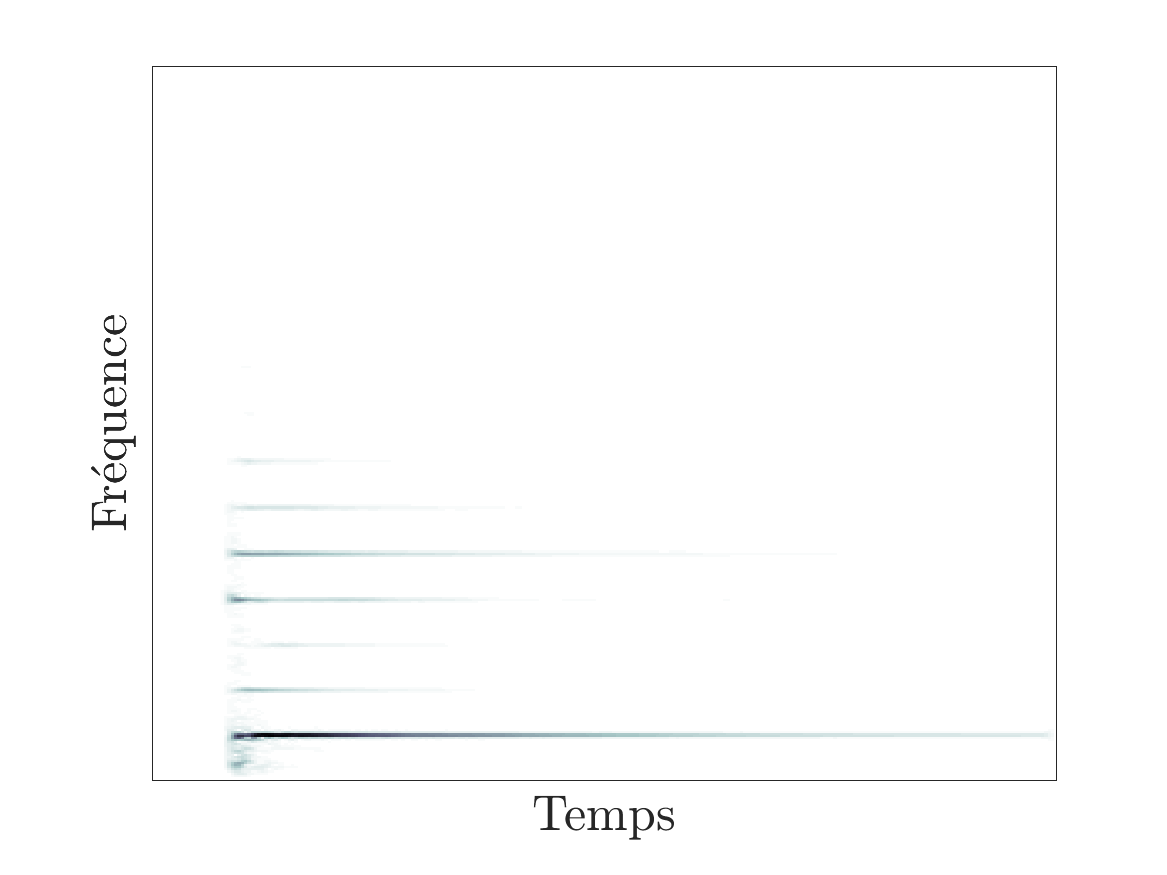
\includegraphics[width=\textwidth]{pianoSpec}
  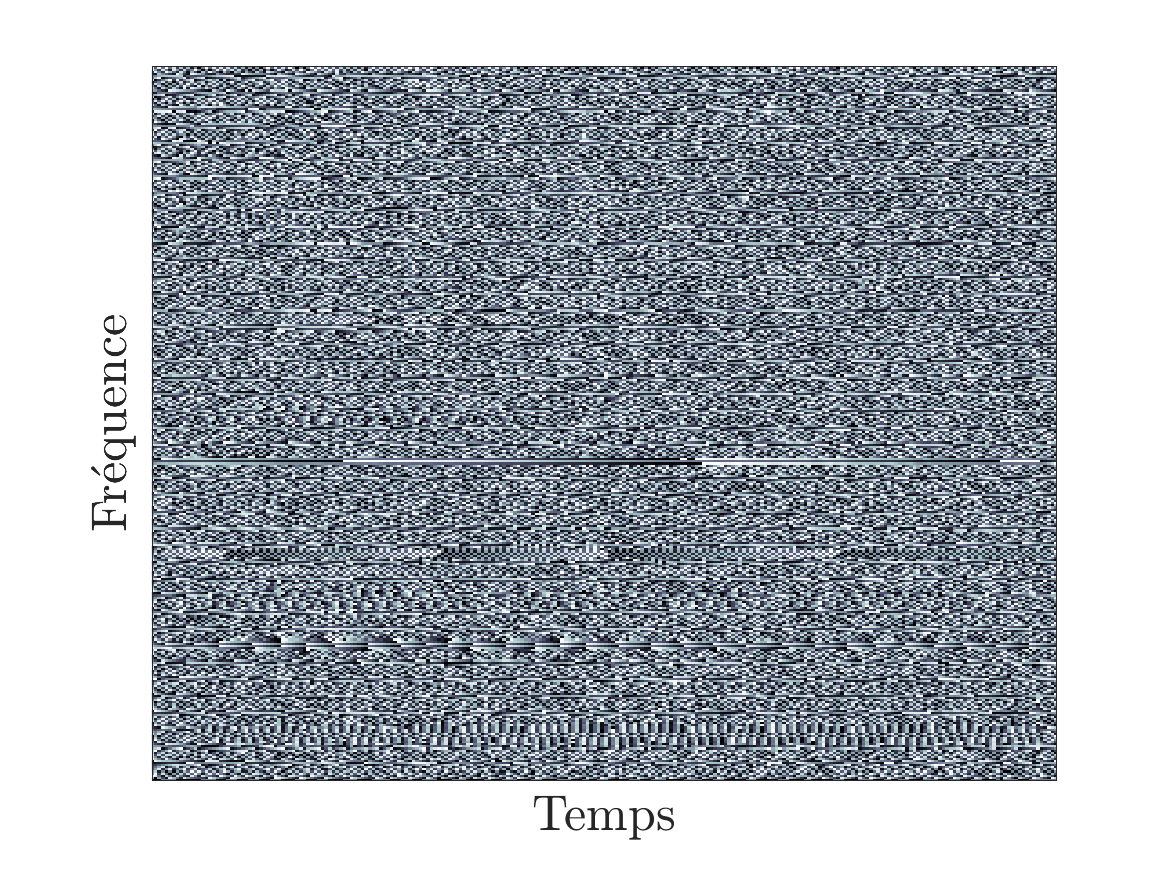
\includegraphics[width=\textwidth]{pianoPhase}
  \caption{Signal temporel ou forme d'onde d'une note de piano.}
  \label{fig:onde}
\end{marginfigure}

Également, le terme modélisation étant fortement polysémique, précisons l'usage qui sera fait du terme \og modèle de son \fg. Un modèle de son est une représentation du signal sonore qui permet de modifier ce signal d'une manière qui soit d'intérêt pour une tâche donnée et ce de manière cohérente avec certaines contraintes motivées par 1) des considérations physiques ou 2) la perception qu'en aurait un être humain. On notera $Pe(x)$, l'opérateur de perception humaine du signal $x$.  Le modèle est utilisé en considérant deux étapes de transformation, respectivement appelées \og analyse \fg et \og synthèse \fg. La phase d'analyse $A$, à partir d'un signal $x$, produit un modèle $X$ et la phase de synthèse $S$ permet, à partir de ce modèle $X$, de produire un signal $\tilde{x}=Sy(An(x))$.

Trois critères d'évaluation émergent alors pour qualifier ce modèle :
\begin{enumerate}
  \item \textbf{fidélité} : un modèle fidèle est capable de ne pas produire d'artefacts. Ce critère peut s'exprimer formellement de la manière suivante : $Pe(x) \sim Pe(\tilde{x})$.
  \item \textbf{expressivité} : un modèle expressif est capable de mettre à disposition des mécanismes de manipulation tels que la modification du modèle produise une modification cohérente de la perception du signal résultant. Ce critère peut s'exprimer formellement de la manière suivante : $Pe(Sy(X')) \sim Pe'(Sy(X))$.
  \item \textbf{versatilité} : un modèle versatile s'applique à tout type de signal sonore d'intérêt, \textit{i.e.} les conditions de fidélité et d'expressivité sont remplies pour tout signal $x$ d'intérêt pour une tâche donnée.
\end{enumerate}
\marginnote{J'évacue ici volontairement la notion d'efficacité, \textit{i.e.} la capacité à modéliser des signaux avec peu de paramètres. Cette notion sera un élément prépondérant d'évaluation par exemple pour un algorithme de compression. De par mon expérience, même si les aspects d'expressivité et d'efficacité peuvent paraître liés de manière formelle, ces deux notions se trouvent à ce jour assez éloignées en pratique.}
\marginnote{
\begin{tikzpicture}[scale=0.8, label distance=1.5mm]
    \coordinate[label=below:Fidélité]  (A) at (0,0);
    \coordinate[label=below:Versatilité] (B) at (4,0);
    \coordinate[label=above:Expressivité] (C) at (2,3.464);
    \draw [line width=1.5pt] (A) -- (B) -- (C) -- cycle;
    \draw [black, fill=black, line width=1.5pt] (2,.3) circle [radius=.1 cm]; % raw
  \end{tikzpicture}
  La forme d'onde est modèle de son versatile et fidèle mais d'une expressivité limitée.
}
Avec ces trois critères d'évaluation, se dessine ici un triangle de contraintes qui nous permettra d'apprécier le compromis inhérent au choix  de chacun des modèles que nous discuterons. Par exemple, la forme d'onde est un modèle versatile et fidèle mais d'une expressivité limitée.

L'intuition ici, largement suivie dans la communauté des sciences des données est que, pour tout processus observable, il existe un modèle de ce processus pour lequel des manipulations basé sur des opérateurs mathématiques simples dans le domaine transformé \og font sens \fg dans le domaine \fg signal \og d'origine. On jugera alors la qualité du modèle par sa capacité à proposer de nouvelles réalisations du processus modélisé qui soient plausibles, c'est-à-dire perceptivement valides. Par exemple, en considérant le signal temporel, on peut aisément manipuler l'intensité perçue en multipliant tout les échantillons par une constante. Ce modèle ne permet par contre pas dans le cas général de manipuler aisément la hauteur perçue.

Cette approche se distingue clairement des approches dites \og modèles physiques \fg qui modélisent explicitement le processus mécanique, la qualité du son étant alors censée être la résultante d'une bonne modélisation du système physique dont la mise en vibration est à l'origine du signal sonore d'intérêt. Le distinguo est ici fait sur l'objet d'intérêt, à savoir que l'on s'intéresse aux propriétés du signal et non celles de la source. Ceci ne veut pas dire que l'on ne puisse pas, avec une approche sciences des données, se focaliser sur le signal d'un type de source sonore en particulier. Mais, dans ce cas, on s'attachera à exploiter les régularités du signal pour motiver notre modèle.

Dans la communauté traitement du signal, on parle souvent de modèle paramétrique, dans le sens où le modèle dispose d'un ensemble réduit de paramètres qui peuvent être explicitement manipulés pour influer sur le son modélisé. L'usage du terme \og paramétrique \fg est néanmoins à mon avis peu clair, et utilisé avec plus ou moins de bonheur dans la littérature. Je préférerai donc à ce terme le distinguo entre \og modèle \fg et \og transformée \fg. Un modèle expose donc pour moi un ensemble de paramètres manipulables, une transformée étant plutôt un outil de description. Ceci n'empêche pas qu'une transformée puisse avoir un modèle sous-jacent, ni que les étapes d'analyse et/ou de synthèse d'un modèle ne se basent sur une ou des transformées.

Précisons maintenant l'intervalle temporel dénommé par \og long terme \fg. Cela désignera ici une durée à partir de laquelle le signal sonore ne peut plus raisonnablement être considérée comme stationnaire.

De par nos connaissances sur les propriétés physiques de l'organe phonatoire, il est par exemple commun de considérer que le signal de parole est localement stationnaire sur un intervalle de 25 ms. Comme on peut le voir sur la Figure \ref{fig:speech} montrant des spectrogrammes de vocalisations humaines\cite{ladefoged2014course}, dès que l'on considère des consonnes, ou lorsque la prosodie évolue de manière conséquente, le signal sonore produit par l'organe vocal n'est plus stationnaire. Il me paraît donc plus juste de motiver ce choix par l'assertion suivante : \og il est raisonnable d'approximer le signal de parole avec un modèle stationnaire par morceaux à partir du moment où ces morceaux sont d'une durée inférieure à 25ms \fg.

\begin{marginfigure}
  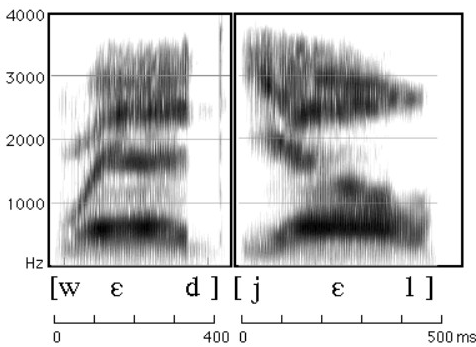
\includegraphics[width=\textwidth]{phonemesCrop}
  \caption{Spectrogrammes de vocalisations humaines.}
  \label{fig:speech} % Issue de l'ouvrage "A Course In Phonetics" de Ladefoged publié en 2006,  http://www.cog.jhu.edu/courses/325-f2004/ladefoged/course/chapter8/figure8.html
\end{marginfigure}

La dénomination \og long terme \fg  étant dépendante du degré de stationarité du signal étudié, il n'est donc pas possible de fixer une durée pour tout type de signaux sonores à partir de laquelle la dénomination \og long terme \fg est appropriée. On considérera néanmoins dans les études discutées dans ce document qu'un intervalle de temps  \og long terme \fg désigne un intervalle de temps supérieur ou égal à la seconde.

\section{ \nmu Typologie sonore} \label{sec:typologie}

Il est bien entendu que même si l'on souhaite que notre modèle soit versatile, on ne souhaite pas nécessairement que notre modèle soit capable de modéliser tout les signaux possibles. On supposera donc que certaines propriétés d'invariance existent, c'est-à-dire que même si une seconde de son échantillonnée à 44kHz est représentée dans $R^{44000}$, les paramètres du modèles\footnote{Ou variables latentes, ou encore code...} évoluent dans un espace de dimension beaucoup plus réduit. Je considère ce postulat raisonnable essentiellement pour des raisons d'observations physiques. En prenant l'exemple du signal de parole, il est bien entendu que le son produit est le résultat d'une interaction complexe entre un ensemble d'éléments qui ont une certaine plasticité. Il en reste néanmoins évident que les déformations possibles de l'ensemble de ces éléments sont bornées.

Dans le but de préciser le domaine d'investigation, je présente ici cinq grandes familles de signaux sonores :
\begin{itemize}
  \item \textbf{parole} : sons voisés <a>, <o> / sons plosifs <pe>, <qe>
  \item \textbf{communication animale} : hululement de chouettes / clics de localisation de chauve souris
  \item \textbf{musique} : chant lyrique / percussions
  \item \textbf{mécanique} : ventilation / marteau piqueur
  \item \textbf{environnementaux} : vent faisant siffler des câbles / gouttes de pluie tombant sporadiquement
\end{itemize}\footnote{Cette typologie est ordonnée par période approximative d'intérêt de la communauté de traitement du signal. Le traitement de la parole a connu un essor dans les années 1970, la bio acoustique un peu plus tard, la musique dans les années 2000 et les signaux environnementaux dans les années 2010.}

Les exemples donnés pour chaque classe sont choisis à dessein pour illustrer une dichotomie présente dans toutes ces classes. Elle qui permettra d'asseoir notre critique des outils de modélisation à notre disposition et d'identifier les challenges majeurs que nous devons relever.

On note donc que certains sons portent une structuration fréquentielle forte et d'autres une structuration temporelle forte\marginnote{Pour un exemple dans le domaine instrumental, voir la Figure \ref{fig:ibm}}. Ces exemples sont volontairement typés pour expliciter le propos, mais la plupart des sons naturels sont une composition de ces deux types de structures. Il est donc nécessaire pour atteindre nos objectifs de disposer d'outils performants pour modéliser conjointement ces deux types de structure.

\section{ \nmu Temps / fréquence} \label{sec:tf}

Lorsque l'on cherche à décrire un son, deux dimensions émergent : l'intensité et la hauteur. Ces deux dimensions étant respectivement intimement liés au volume et à la fréquence, il est normal de constater que la plupart des modèles de son permettent de manipuler ces deux dernières quantités et ce, de manière dynamique \textit{i.e.} au cours du temps.

En supposant le signal sonore stationnaire sur l'intervalle d'observation, l'outil privilégié pour ce faire est la transformée de Fourier discrète (TFD). Cette transformée projette le signal sur une base d'exponentielles complexes:
\begin{eqnarray}
  S[m] &=& \sum_{n=0}^{N-1} s[n] e^{\frac{-2j \pi nm}{N}} \\
  s[n] &=& \frac{1}{N} \sum_{m=0}^{N-1} X[m] \cdot e^{\frac{ 2 j \pi m n }{N}}
\end{eqnarray}

Ces exponentielles formant une base, il est possible de revenir au signal d'origine (ITFD(TFD(x))=x). Cette transformée est donc inversible, mais n'est pas à échantillonnage critique car $s\in \mathbb{R}$  et $S \in \mathbb{C}$. On calcule la transformée de Fourier de manière efficace grâce à des algorithmes de transformée de Fourier rapides qui exploitent, pour le plus connu d'entre eux, des longueurs de supports en puissance de deux.

En considérant le module de cette transformée, on manipule directement l'intensité du son à la fréquence donnée. Le spectre de phase est lui souvent négligé dans les modèles, car il est beaucoup plus difficile à interpréter. Ceci constitue un handicap majeur pour tout les modèles de sons basés sur la transformée de Fourier car cela, comme cela sera discuté dans la suite, pose bien souvent une limite sur la propriété de fidélité, le module et l'exposant étant mathématiquement intrinsèquement lié. Pour exemple, la Figure \ref{fig:phase} montre le spectre de phase d'une note de piano. Pour ce cas simple avec une bonne parcimonie et une structure temporelle élevée, des régularités sont observables aux fréquences des harmoniques de la note de piano. Pour des scènes plus complexes, l'interprétation du spectre de phase devient ardue.

\begin{marginfigure}
  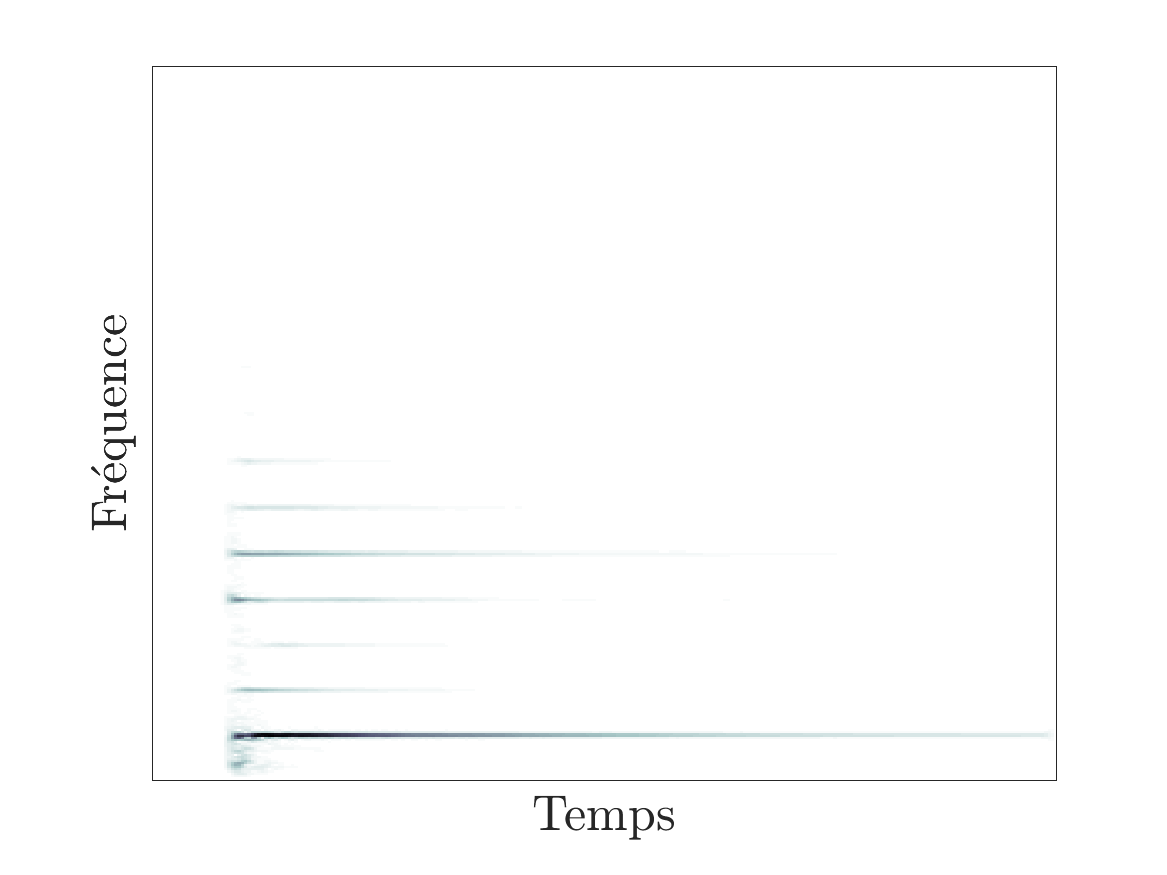
\includegraphics[width=\textwidth]{pianoSpec}
  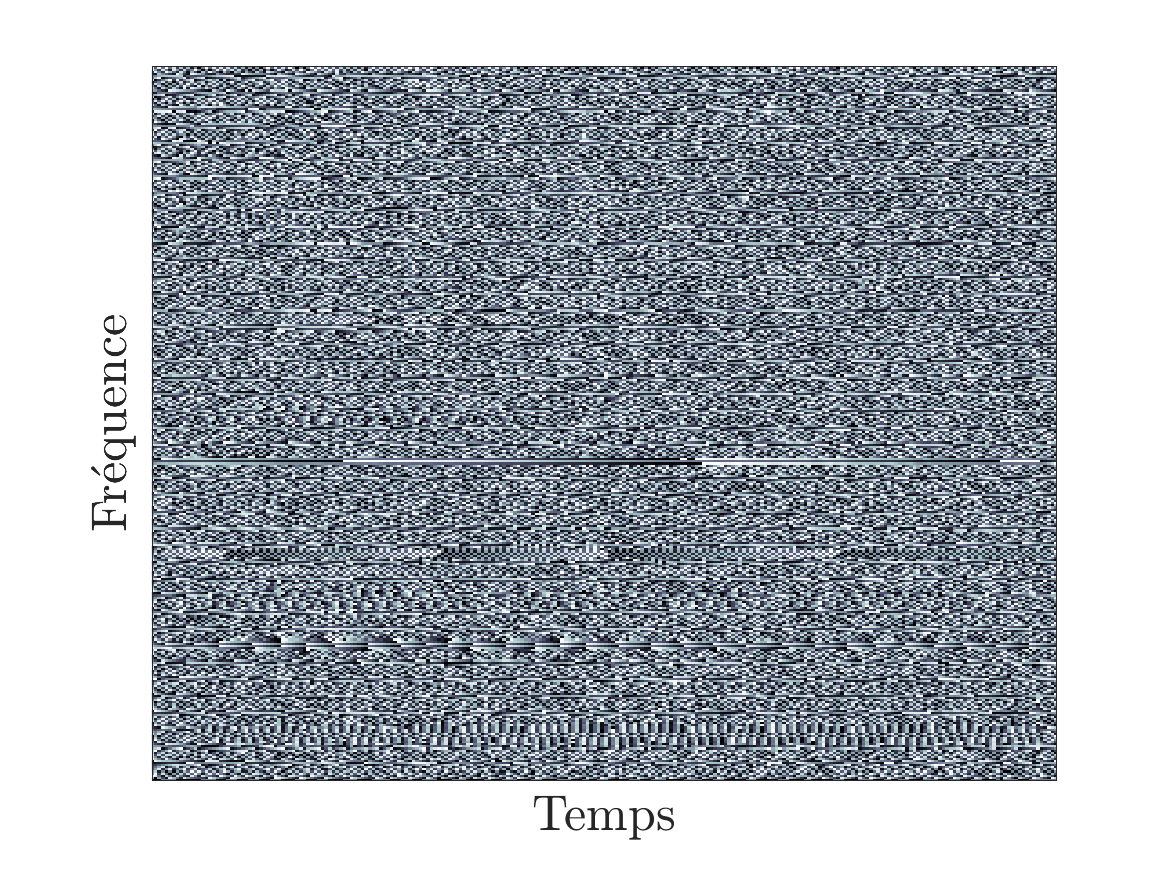
\includegraphics[width=\textwidth]{pianoPhase}
  \caption{Spectrogramme d'amplitude, et de phase d'une note de piano.}
  \label{fig:phase}
\end{marginfigure}

En considérant qu'une partie des sons que l'on cherche à modéliser ont une structure temporelle forte, on s'intéresse à l'estimation des paramètres de composantes périodiques simples, les sinusoïdes. Considérons pour cela un premier signal \og éprouvette \fg constitué d'une sinusoïde de fréquence et d'amplitude constante:
\begin{equation}
  s_s[n] = a_s sin(2\pi f_s/f_e + \phi_s)
  \label{eq:sin_toy}
\end{equation}
Les paramètres d'amplitude et de fréquence de cette composante s'estiment aisément grâce au spectre de Fourier de ce signal :
\begin{eqnarray}
  \hat{f_s} &=&  \frac{M}{N} . f_e\\
  \hat{a_s} &=& S_s[M].3333
\end{eqnarray}
avec
\begin{equation}
  M = \argmax_m | S_s[m] |.
  \label{eq:sin_toy_select}
\end{equation}

Dans le cas de plusieurs sinusoïdes, on remplacera l'équation \ref{eq:sin_toy_select} par une sélection de maxima locaux dans le spectre de puissance et on considèrera l'usage d'une fenêtre de type co-sinusoïdale (hamming, hann, ...) pour améliorer la localité fréquentielle de la transformée\cite{harris1978use}. En effet, considérer le signal sur un intervalle de temps fixé par la largeur de la trame revient implicitement à fenêtrer le signal par une fenêtre rectangulaire qui a des propriétés spectrales non désirables dans le cas multi composantes. Avec des fenêtres co-sinusoïdales, le lobe principal s'élargit, d'où une perte locale de résolution, mais permet de réduire considérablement l'importance des lobes secondaires, ce qui s'avère indispensable dans un contexte multi composantes.
\marginnote{
   \begin{center}
   (a) \\
   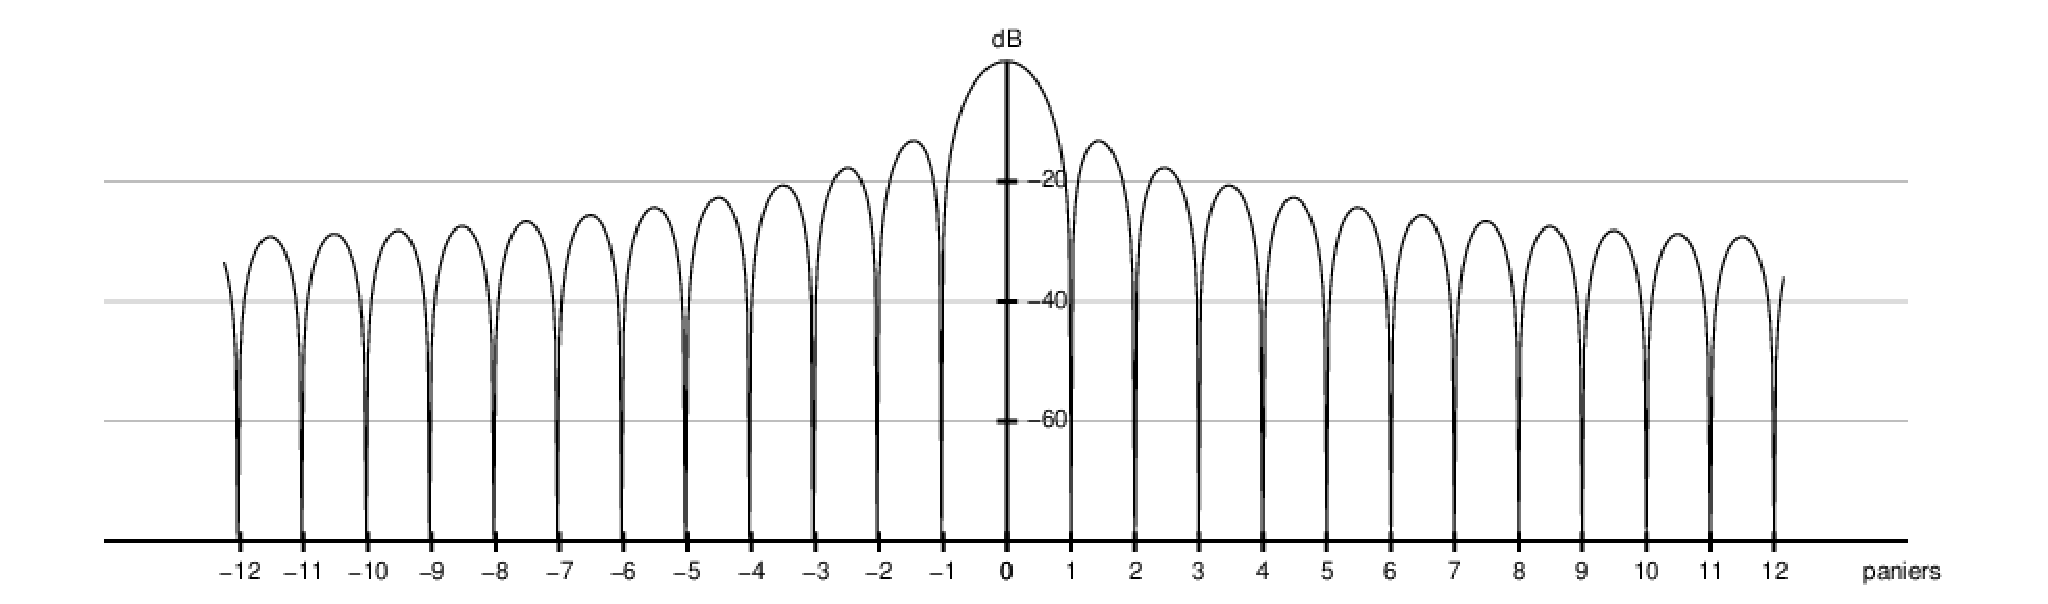
\includegraphics[width=.5\textwidth]{s-rectangularFr} \\
   (b) \\
  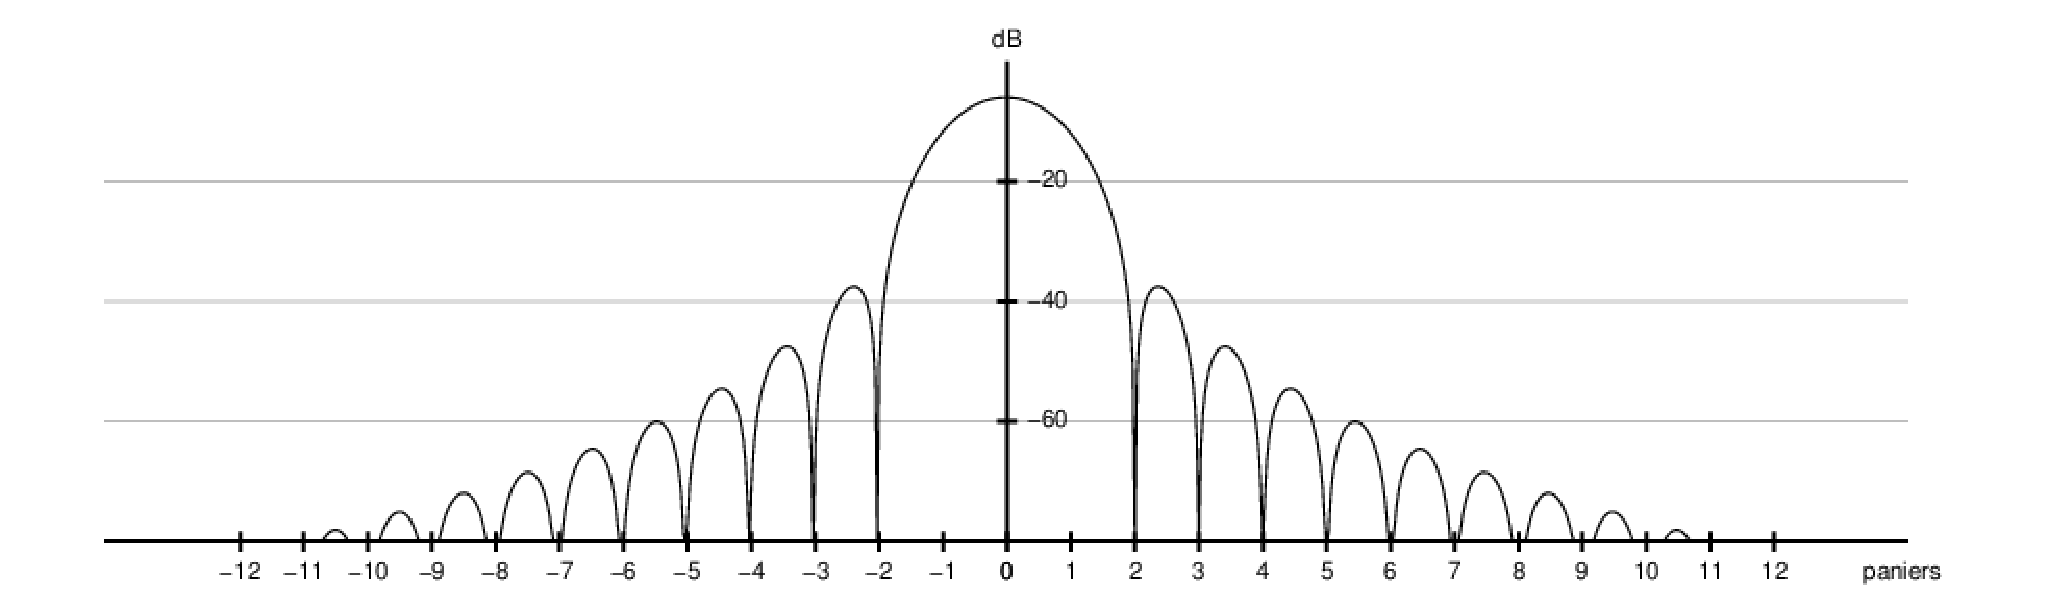
\includegraphics[width=.5\textwidth]{s-hannFr}
 \end{center}
Spectre d'amplitude de la fenêtre rectangulaire (a), et de la fenêtre de Hann (b).
}

On peut améliorer la précision de ces estimations en réduisant le pas de quantification de l'axe fréquentiel. On utilise pour cela la technique du "zero padding", qui consiste à concaténer une série de valeurs nulles au signal observé avant d'opérer la transformation. La transformée s'opérant alors sur plus de points, sa précision en est augmentée.

Un large échantillon de méthodes sont disponibles pour améliorer la précision de ces estimations par d'autres moyens moins directs, comme  celles basées sur le réassignement~\cite{auger1995improving} qui étudient les relations entre le spectre du signal fenêtré et le spectre du signal fenêtré par la dérivée de la fenêtre, ou encore les méthodes basées phase qui étudient les relations entre le spectre du signal et celui de sa dérivée, dont nous avons pu montrer l'équivalence théorique et numérique~\cite{lagrangeJaes07}.

Il est important de bien garder en mémoire que seule la précision est augmentée, la résolution restant dépendante de la largeur du support temporel.  Augmenter l'intervalle d'observation va donc non seulement influer sur la précision, mais également sur la résolution de la transformée. Ainsi, deux sinusoïdes de fréquences proches ne pourront être \og résolues \fg, c'est-à-dire que leurs paramètres pourront être estimés en observant directement le spectre d'amplitude uniquement par l'extension suffisante du support temporel de la transformée.

Considérons un autre signal \og éprouvette \fg constitué cette fois ci d'un dirac :
\begin{equation}
  s_d[n] = \begin{cases}
    a_d \text{ si } n=n_d \\
    0 \text{ sinon}
\end{cases}
\end{equation}
L'estimation du paramètre d'amplitude $a_d$ et de sa position temporelle $n_d$ est triviale dans le domaine temporel :
\begin{eqnarray}
  \hat{n_d} &=&  \argmax_n | s_d[n] | \\
  \hat{a_s} &=&  s_d[\hat{n_d}].
\end{eqnarray}

Cette dernière est par contre beaucoup plus difficile à estimer dans le domaine spectral, du fait du caractère non stationnaire du signal analysé.

Pour palier au caractère non stationnaire à long terme de la plupart des signaux naturels, il est courant d'utiliser la transformée de Fourier à court terme (TFCT). Son principe est d'effectuer une série de transformée de Fourier, chacune sur des fenêtres espacées dans le temps:
\begin{equation}
X[m, t] = \sum_{n = - \infty}^{\infty} x[n] w[n-t] e^{\frac{-2 j  \pi m n}{N}}
\end{equation}
où $w$ est la fenêtre d'observation.

\marginnote{
\begin{tikzpicture}[scale=0.8, label distance=1.5mm]
  \coordinate[label=below:Fidélité]  (A) at (0,0);
  \coordinate[label=below:Versatilité] (B) at (4,0);
  \coordinate[label=above:Expressivité] (C) at (2,3.464);
  \draw [line width=1.5pt] (A) -- (B) -- (C) -- cycle;
  \draw [olive, fill=olive, line width=1.5pt] (1.8,.8) circle [radius=.1 cm]; % spec
  \end{tikzpicture}
  Le spectrogramme est à ce jour le compromis le plus apprécié.
}

En prenant le spectre de magnitude de la TFCT, on obtient le bien connu spectrogramme, un outil de manipulation et de visualisation qui trouve son utilité dans de nombreux domaines d'application. L'espoir ici est que les erreurs de modélisation des non stationarités du signal seront négligeables du fait du faible support temporel des fenêtres sur lesquels on applique successivement la TFD. Dans le cas où les fenêtres se recouvrent de moitié, on peut utiliser la transformée en cosinus discret modifiée (TCDM) pour conserver un échantillonnage critique\cite{princen1986analysis}.

En considérant la TFCT, il est alors possible de construire un estimateur \og spectral \fg de la position temporelle de notre dirac :
\begin{equation}
\hat{n_d} = \argmax_t \sum_m X(m, t)
\end{equation}
\'A condition d'utiliser une fenêtre \fg à rampe \og, on peut améliorer la précision temporelle de cet estimateur en réduisant le recouvrement entre fenêtres. La encore, il s'agit d'une amélioration de la précision et non de la résolution. Seule la réduction de l'intervalle d'observation permettra de résoudre la position temporelle de deux diracs proches.

Au travers de ces deux exemples, on voit qu'il est possible d'améliorer dans une certaine mesure la précision des estimations de certaines quantités d'intérêt que l'on peut faire à partir d'un plan temps/fréquence obtenu grâce à la TFCT, mais que les résolutions temporelles et fréquentielles reste conflictuellement contraintes par la taille de la fenêtre choisie. On parle de variables complémentaires pour le temps et la fréquence, au même titre que la position et la quantité de mouvement en mécanique.

Le problème se corse alors sensiblement lorsque l'on considère des signaux qui possèdent une localité temporelle et fréquentielle, ce qui est le cas de la plupart des signaux sonores naturels\marginnote{Un exemple iconique étant la note de piano dont la qualité s'exprime autant du côté de la localité temporelle (netteté de l'attaque) que de la localité fréquentielle (pureté des harmoniques).}.

Il paraît alors naturel de considérer des approches à résolution multiples. Tout le problème consiste alors à trouver une représentation qui maximise le potentiel apporté par la multi résolution en terme de fidélité tout en minimisant la perte en expressivité. En effet, la manipulation de données non régulièrement échantillonnées ou recopiées sous diverses formats, sont un frein à l'aisance de manipulation.

Pour parvenir à une représentation à résolution multiple, l'approche la plus simple conceptuellement consiste à \og effectuer \fg plusieurs DFT de largeur de fenêtre différentes, et ce à intervalle régulier. Cette technique peut se révéler utile dans le cas d'inspection de données ou de prises de décision. Il est par exemple courant, de procéder à des fusions ensemblistes de classifieurs d'architectures équivalentes effectuant leurs prédiction à partir de représentations spectrales de résolution différentes. Dans le cas d'un modèle de son, cela induit malheureusement une perte inacceptable en manipulabilité du fait de la perte d'unicité de la représentation.

Pour éviter cette perte, il est nécessaire de baser notre modèle sur une représentation qui soit à même de partager judicieusement le plan temps / fréquence de manière à mitiger au mieux la contrainte posée par le principe d'incertitude. Un immense travail de la communauté de traitement du signal a été de concevoir ce type de transformée, connue maintenant sous le nom de transformée en \og ondelettes \fg.\cite{mallat1989theory}.

Même si les travaux théoriques dans ce domaine ont permis d'ouvrir considérablement les possibilités en terme de conception, je me  tiendrai ici à la forme la plus courante en traitement du signal qui consiste en une construction d'un banc de filtre dyadique à facteur de qualité constant. Ce banc de filtre est constitué d'un ensemble filtres passe bande à l'octave, \textit{i.e.} la fréquence de coupure supérieure est égale à deux fois la fréquence de coupure inférieure. On obtient alors un pavage alternatif du plan temps / fréquence. Du fait du principe d'incertitude, les paniers ont la même aire, mais le rapport entre résolution fréquentielle et temporelle est optimalement adapté.

\marginnote{
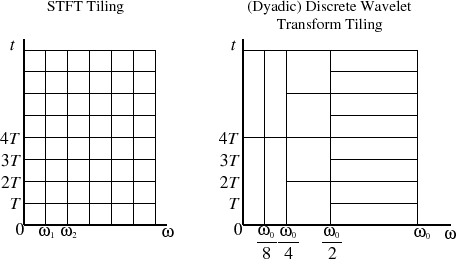
\includegraphics[width=\textwidth]{waveletBins.png}
Pavage du plan temps/fréquence pour le spectrogramme (a) et la transdformée en ondelettes (b).
}


En considérant que le banc de filtre est construit de manière itérative en partant des hautes fréquences, et en notant que le signal observé est d'une durée limitée, une partie du spectre en basse fréquence ne peut être capturé. On ajoute alors un filtre passe bas dit \og de terminaison \fg qui permet de préserver l'unicité de la représentation. Ce dernier filtre est souvent appelé \og fonction d'échelle \fg. Les sorties de ce banc de filtres peuvent être ensuite re-échantillonnées à une fréquence de Nyquist correspondante à la largeur de la bande d'octave du filtre considéré% QUID DU FILTRE DE TERMINAISON ?
. Comme le montre les travaux pionniers en ce domaine\cite{kronland1987analysis}, l'application de la transformée en ondelettes paraît avoir d'excellentes propriétés pour le traitement de l'audio, en particulier cette capacité à proposer une analyse multirésolution en préservant la propriété d'unicité.

\marginnote{
\begin{tikzpicture}[scale=0.8, label distance=1.5mm]
  \coordinate[label=below:Fidélité]  (A) at (0,0);
  \coordinate[label=below:Versatilité] (B) at (4,0);
  \coordinate[label=above:Expressivité] (C) at (2,3.464);
  \draw [line width=1.5pt] (A) -- (B) -- (C) -- cycle;
  \draw [brown, fill=brown, line width=1.5pt] (2.4,.6) circle [radius=.1 cm]; % wavelets
  \end{tikzpicture}
  Les modèles de sons basées sur la transformée en ondelettes sont en théorie plus versatile grâce à la multirésolution, mais peu de travaux démontrent leur expressivité.
}

Quelques décennies plus tard, on peut faire le constat que l'utilisation de la transformée en ondelettes reste marginale en traitement de l'audio. Dépasser ce constat pour amener des éléments concrets nécessiterait une étude approfondie qui sort du cadre de cet exposé. On peut néanmoins avancer quelques éléments de réflexion. Une première explication peut être que les fonctions de bases de la transformée en ondelettes, \textit{i.e.} les réponses impulsionnelles des filtres passe bande ont des formes particulièrement irrégulières, non adaptées à l'audio. On peut en effet aisément retenir cet argument pour des ondelettes de Daubechies de faible longueur, mais devient moins recevable pour des longueurs plus élevées, ou pour les ondelettes de morlet. Cet argument pourrait néanmoins expliquer pourquoi cette transformée à plutôt pris son essor dans le domaine du traitement d'image, où les discontinuités sont beaucoup plus fortes que pour les signaux sonores. En effet chaque contour d'un objet amène une discontinuité importante dans l'espace couleur, qui, dans le cas de la reconnaissance apporte des éléments d'interprétation très importants, et, dans le cas du codage, se doit d'être représenté en détail, sous peine d'engendrer des artéfacts de type \og lissage \fg très pénalisant.

Une seconde explication, finalement peut être plus déterminante, peut avoir trait à la manipulabilité de la transformée. L'interprétation  du spectrogramme est intuitive et permet une manipulation fine du contenu spectral d'un signal audio par des opérations de masquages par exemple, voir la section dédiée à l'\nameref{sec:asa}. L'échantillonnage non régulier en temps et en fréquence de la transformée en ondelettes ne simplifie pas l'expression des transformations que l'ont souhaitent généralement opérer (transposition, étirement, ...). La version filtrée pour obtenir un échantillonnage régulier en temps est plus appropriée, mais au prix de la perte de toute notion de multi-résolution.

% \begin{marginfigure}
%   (a) \\
%   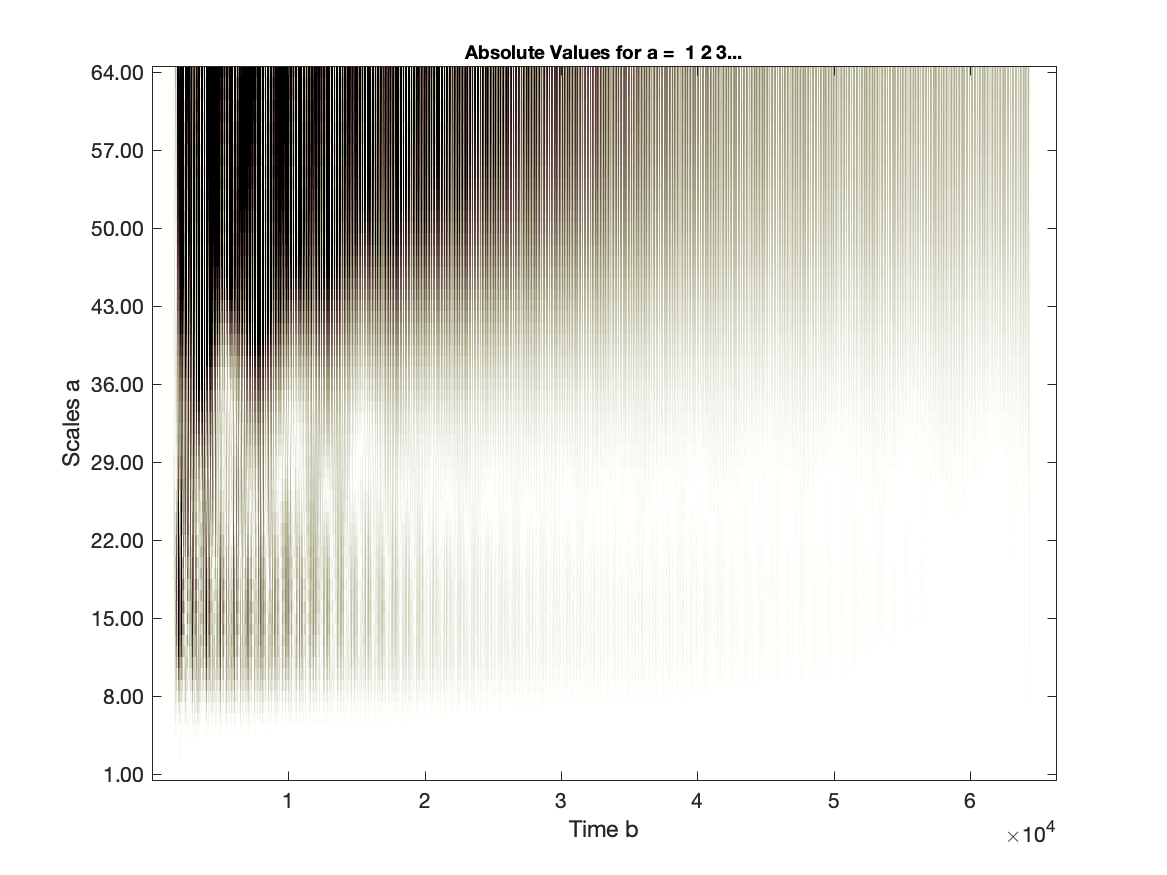
\includegraphics[width=\textwidth]{pianoCwt} \\
%   (b) \\
%   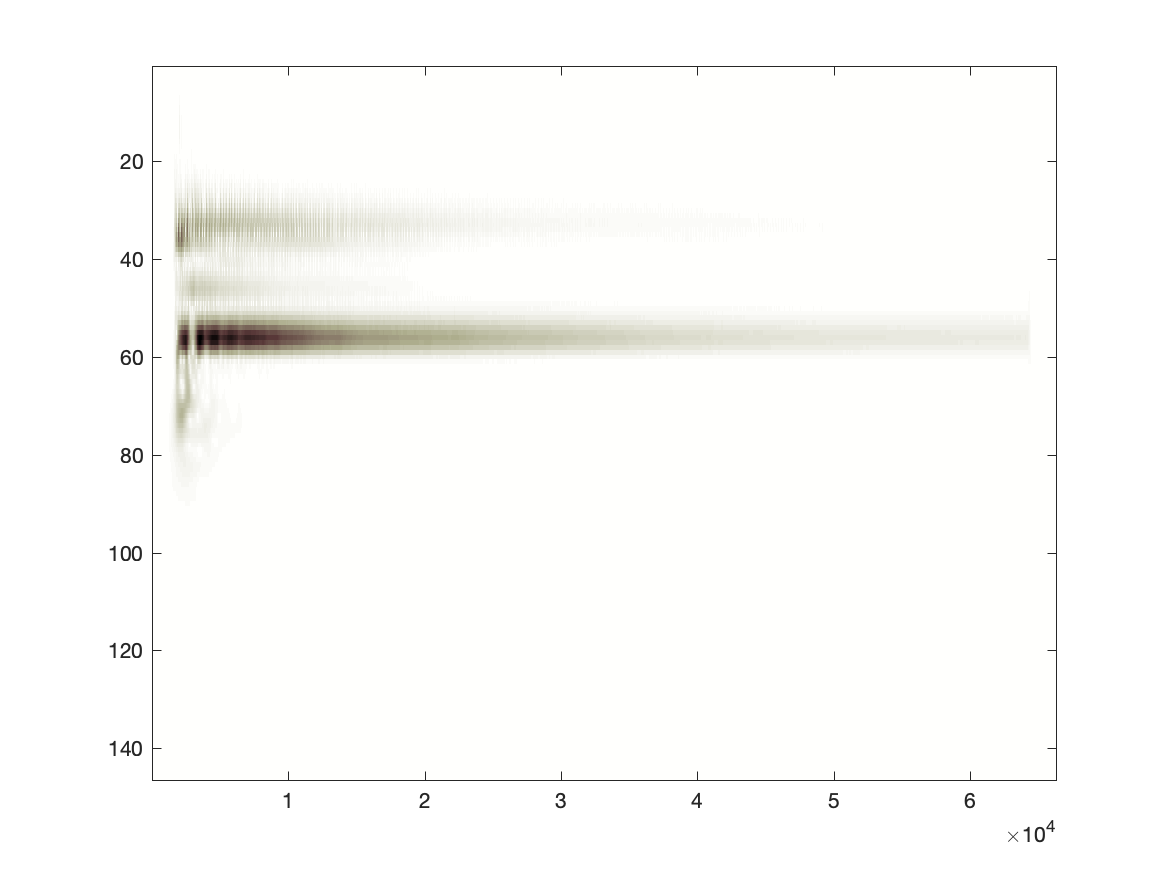
\includegraphics[width=\textwidth]{pianoSca}
%   \caption{transformée en ondelettes (a) et scalogramme (b) d'une note de piano.}
% \end{marginfigure}

En tout état de cause, dans le domaine de l'audio, la grande majorité des systèmes de traitement considère une représentation de type TFCT, avec des paramètres de résolution et de précision constants, adaptés à la tâche. Dans les applications de codage, on trouve des mécanismes à résolution multiple de type alterné, implantés grâce des TCDM à plusieurs largeurs de support\cite{brandenburg1999mp3}. Au sein du codeur, une heuristique détermine parmi les résolutions possibles, la résolution la plus adaptée au vu du signal contenu dans l'intervalle d'observation considéré. Cet échantillonnage non régulier de l'axe temporel permet une meilleure fidélité et flexibilité si l'heuristique est adaptée, ceci au détriment de la manipulabilité, le plan temps/fréquence induit étant non régulier, ce qui n'est généralement pas un facteur limitant dans des chaînes de codage.

On considère donc ici que dans l'intervalle d'observation, une source sonore est dominante et que le type de source est structurée soit de manière temporelle soit de manière fréquentielle. Dans le cas d'un contenu polyphonique avec une structure à la fois en temps et en fréquence, cette approche se révèle bien entendu inopérante. La définition d'une méthode d'analyse/synthèse multirésolution reste donc, avec les éléments présentés ici, un champ de recherche encore largement ouvert.

\section{ \nmu Sinusoïdes à court terme}  \label{sec:sct}

Lorsque l'on observe un spectrogramme un instrument de musique tonal, comme celui d'une note de piano (Figure \ref{fig:phase}), il apparaît clairement que l'énergie est concentrée en un ensemble réduit de zones fréquentielles. On dit que ces signaux sont parcimonieux en fréquence. C'est, dans une certaine mesure le cas de la parole\marginnote{En tout cas, il est clair que la \og charge sémantique \fg est portée par cette partie du signal de la parole, comme le montre les exemples de "sine-wave speech", un nombres réduit de sinusoïdes judicieusement placées aux zones de résonances formantiques suffisent à rendre le signal intelligible \url{http://webpages.mcgill.ca/staff/Group2/abregm1/web/downloadstoc.htm\#23}.}.

En suivant cette observation, on peut modéliser chaque zone de forte énergie du plan temps/fréquence par une composante sinusoïdale à court terme. Pour cela, il est commun d'identifier des maxima locaux dans chaque spectre du spectrogramme pour identifier un ensemble de \og pics spectraux \fg, ou \og atomes \fg temps fréquence. On obtient alors le modèle de son suivant :
\begin{equation}
  S_{ct}(t) = \sum_{c=1}^{C_t} a(c,t) sin(2 \pi f(c,t) t + \phi(c,t))
\end{equation}

Les paramètres de fréquence, d'amplitude, et de phase de chaque atome peuvent être estimées grâce aux techniques évoquées dans la section précédente. Même si cette technique est motivée par la parcimonie, elle se révèle très robuste à la réduction de cette dernière pour peu que le nombre de composante soit suffisant. En effet, l'expansion de Karhunen Loeve de signaux bruités montre qu'une représentation sinusoïdale de ce type de signaux est valide, à condition que les pics soient suffisamment nombreux et de fréquence suffisamment proche pour que la densité spectrale de puissance dans ces zones varie lentement dans le temps\cite{mcaulay}. Le nombre de composantes par intervalle de temps $C_t$ est donc un facteur déterminant. En pratique, dans un compromis favorisant la fidélité et la versatilité au détriment de l'expressivité, on choisira $C_t$ en fonction de contraintes de complexité, \textit{i.e.} le plus grand nombre possible.

%La précision de ces estimations peut être améliorer par des techniques de sur échantillonage en fréquence et en temps, au détriment du coût de calcul. Ceci étant dit, les limites de cette technique sont bien illustrés dans la figure suivante :

% voice_1024_512.eps

% Ce problème d'estimation dépassant largement la problématique de la modélisation du signal audio, un effort conséquent d'amélioration des ces estimateurs a été effectué par la communauté de traitement du signal. Les approches les plus efficaces et les plus élégantes pour ce faire se basent sur des relations entre les paramètres spectraux de plusieurs transformées de Fourier effectuées après différents traitements du signal observé. La technique du reassignement spectral\cite{auger1995improving} considère le rapport entre la DFT du signal fenêtré et la DFT du signal fenêtré par la dérivée de la fenêtre :
% \begin{equation}
% t
% \end{equation}
% En considérant le rapport de la DFT du signal et celle de la DFT de la dérivée du signal, on obtient une autre série d'estimateurs. On a prouvé l'équivalence théorique de ces dernières à la technique du réassignement, supportée par des expérimentations montrant des performances similaires\cite{lagrangeJaes07}.

Dans un objectif d'expressivité, il est important que l'observation  soit en adéquation avec le modèle utilisé, c'est-à-dire que les composantes sinusoïdales modélisent des composantes quasi-périodiques présentes dans le signal analysé. En effet, même si une partie bruitée du signal peut être raisonnablement modélisée avec des composantes sinusoïdales de fréquence proches et de phase arbitraire, il sera difficile avec cette modélisation de préserver une bonne qualité d'écoute lors de la manipulation de ce modèle.

Il convient donc d'être à même de sélectionner parmi les composantes candidates, celles qui sont les plus appropriées en fonction de critères dits de \og sinusoidalité \fg. Une manière de faire consiste à corréler, pour chaque pic candidat, sa réponse fréquentielle à celle du spectre d'une sinusoïde dont les paramètres sont résultant du processus d'estimation~\cite{peak-selection}. Le degré de corrélation permet alors de quantifier la pertinence du modèle vis-à-vis de l'observation. Une étude comparative semble montrer l'intérêt de cette approche en pratique~\cite{wells2010comparative}. Dans cet algorithme, les références au modèle sont ici construites dynamiquement mais peuvent aussi être échantillonnées. On se rapproche alors du principe des algorithmes de poursuite de sous espaces.

Le principe ici est de s'affranchir des contraintes de la base de Fourier en disposant d'un (très) large dictionnaire d'atomes redondants et de déterminer la combinaison optimale de ces atomes permettant de réduire l'erreur d'approximation. L'algorithme "Matching Pursuit" (MP) proposé par Zhang et Mallat\cite{mallat1993matching} permet de résoudre efficacement ce problème en considérant un algorithme glouton, où, itérativement, l'atome mis à l'échelle ayant la meilleure corrélation avec le signal résiduel (égal au signal d'origine au début de l'algorithme) est sélectionné. Il faut remarquer que l'application de cet algorithme à des signaux musicaux peut poser des problèmes, dont certains ont été étudiés par Rémi Gribonval et ses collaborateurs\cite{gribonval1996sound}. %Par exemple, dans le cas de signaux non stationnaire en amplitude, l'algorithme aura tendance à construire des approximations non satisfaisantes.

\begin{marginfigure}
  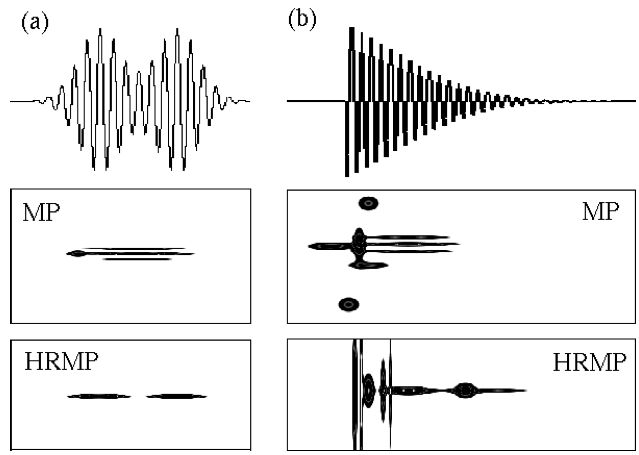
\includegraphics[width=\textwidth]{gribonval.png}
  \caption{Deux composantes sinusoïdales dont l'amplitude est modulée a) sinusoïdalement, b) exponentiellement et décompositions par deux algorithmes de poursuite.}
  \label{fig:gribonval}
\end{marginfigure}

La figure \ref{fig:gribonval} illustre deux cas typiques de ce type de non stationarité rencontrés dans les signaux musicaux. Le premier consiste en une composante sinusoïdale dont l'amplitude est modulée de manière sinusoïdale. C'est une modulation typique d'un tremolo. Le second consiste en une composante sinusoïdale dont l'amplitude est modulée exponentiellement. C'est une modulation typique d'une corde frappée ou pincée comme le piano ou le clavecin.

Dans le cas a), l'algorithme MP identifie d'abord une composante avec un support temporel couvrant l'intégralité du signal. Deux autres composantes viennent ensuite annuler certaines parties de cette première. Dans le cas b), le changement abrupt d'énergie étant difficilement modélisable aves les fonctions de base à disposition, de nombreuses composantes d'annulation sont nécessaires, amenant à un effet de pré écho, l'énergie ajoutée n'étant que partiellement enlevée. Pour palier à ces problèmes, des contraintes de non negativité ont été proposé pour améliorer l'algorithme de poursuite (HRMP). En réduisant les contributions destructives, \textit{i.e.} enlever de l'énergie amené par des atomes sélectionnés mais non présente dans le signal d'origine, cette approche est plus efficace au sens où l'énergie globale des atomes (somme des enveloppes des atomes) est plus faible, cas a) et plus fidèle cas b).

Il est difficile de critiquer ces approches de poursuites dans le sens où leur pertinence vis à vis de la tâche va grandement dépendre du degré de pertinence du dictionnaire choisi. On notera tout de même que ces approches sont construites avec un objectif d'appromixation et non d'identification. Par exemple dans le cas (a), les deux algorithmes de poursuites sont tout deux à même de fournir une bonne approximation du signal, mais \og n'identifie \fg pas le phénomène, le dictionnaire n'ayant pas ce type de forme à disposition. Dans une application de type codage, on préfèrera sans doute la seconde approximation pour des raisons d'efficacité de la représentation. Pour ce qui de la notion d'expressivité, le choix entre les deux modèles seront une affaire de compromis en fonction du type de manipulation souhaité.

On se trouve donc avec un compromis de modèle favorisant la fidélité et la flexibilité, au détriment de l'expressivité. Il est en effet difficile, dans le cas d'un dictionnaire très largement redondant de déterminer des fonctions simples de manipulation.

\marginnote[-15\baselineskip]{
\begin{tikzpicture}[scale=0.8, label distance=1.5mm]
    \coordinate[label=below:Fidélité]  (A) at (0,0);
    \coordinate[label=below:Versatilité] (B) at (4,0);
    \coordinate[label=above:Expressivité] (C) at (2,3.464);
    \draw [line width=1.5pt] (A) -- (B) -- (C) -- cycle;
    \draw [cyan, fill=cyan, line width=1.5pt] (1.6,1.2) circle [radius=.1 cm]; % sct
  \end{tikzpicture}
  Les modèles sinusoïdaux à court terme sont des modèles de son avec une expressivité améliorée par rapport au spectrogramme au prix d'une perte relative en versatilité et fidélité.
}

%Ces approches, comme la transformée en ondelettes, ont trouvés application plutôt dans le domaine du traitement de l'image, où le caractère hautement non stationnaire des transitions entre objets sont très mal approximé par des fonctions régulières comme celle de Fourier.

\section{ \nmu Sinusoïdes à long terme}  \label{sec:slt}

L'approche court terme effectue des observations discrètes d'un processus de production sonore qui lui est par essence continu. Dans le cas de nombreux instruments de musique, il est raisonnable de considérer que ce processus continu est approximable par une somme de sinusoïdes dont les paramètres varient \textsl{lentement} dans le temps. Une variation lente s'entend ici de l'ordre de la dizaine de Hertz. Dans ce cas, le modèle sinusoïdal à long terme est particulièrement à propos. Ce modèle peut s'écrire comme suit :
\begin{equation}
\mathcal{L}=\bigcup_{p=1}^{P}\left\{\mathcal{P}_{p}\right\}
\end{equation}
Chaque composante est appelée un \textsl{partiel} pour des raisons historiques. En effet, ce modèle a été appliqué originellement à des sources monophoniques

Ce modèle est particulièrement expressif car il permet des modifications du signal d'intérêt comme la translation, la transposition, ou encore l'étirement, simplement en manipulant les paramètres. Ces transformations sont de plus de faible coût, les paramètres étant échantillonnés à une fréquence environ 1000 fois plus faible que le signal audio-numérique. Le processus de synthèse est aisé à mettre en oeuvre avec les moyens computationels actuels. Dans le cas d'un très grand nombre de composantes, des algorithmes de "pruning" perceptuels peuvent être mis en place\cite{lagrangeDafx01}.
L'étape d'analyse, \textit{i.e.} l'estimation des paramètres à partir d'un signal sonore est par contre, particulièrement ardue.

\begin{figure*}
  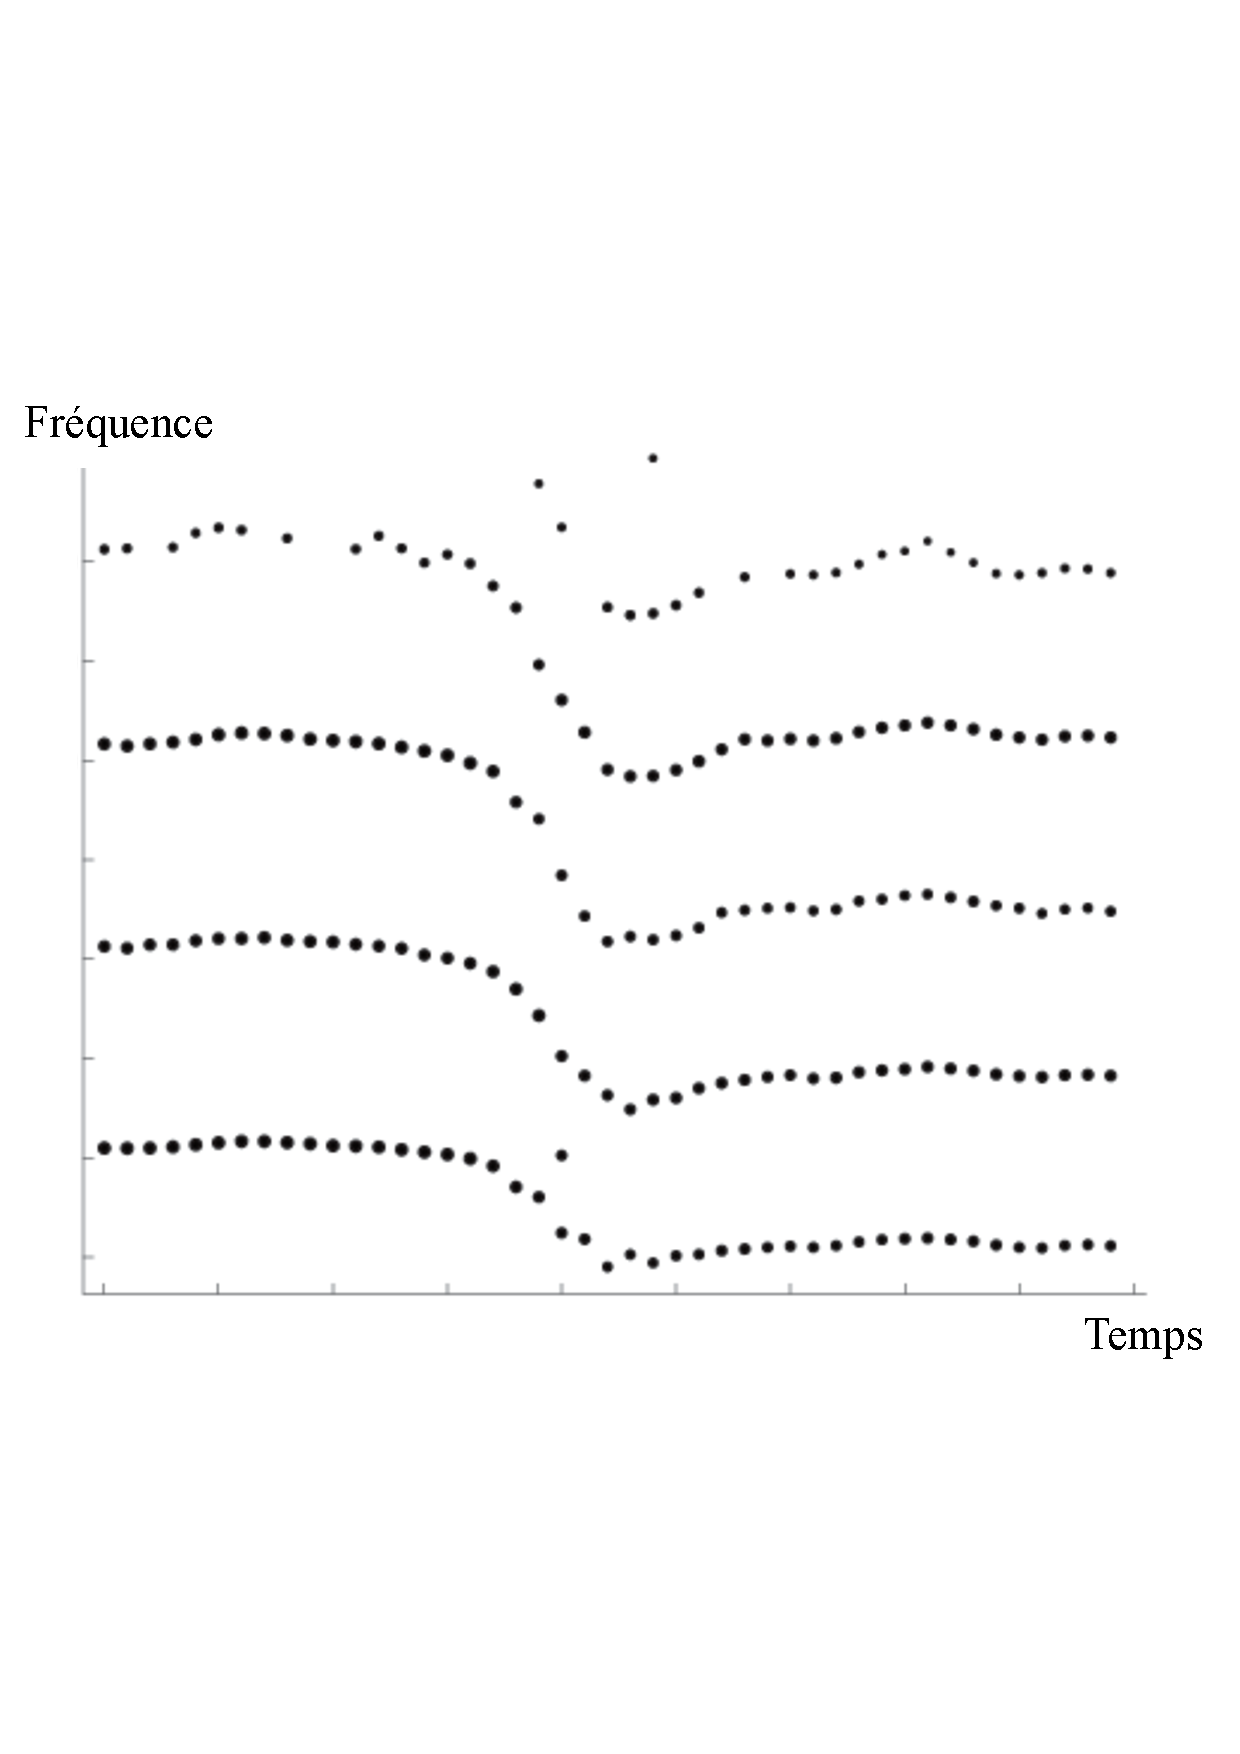
\includegraphics[width=.3333\textwidth]{voice_1024_512xp}
  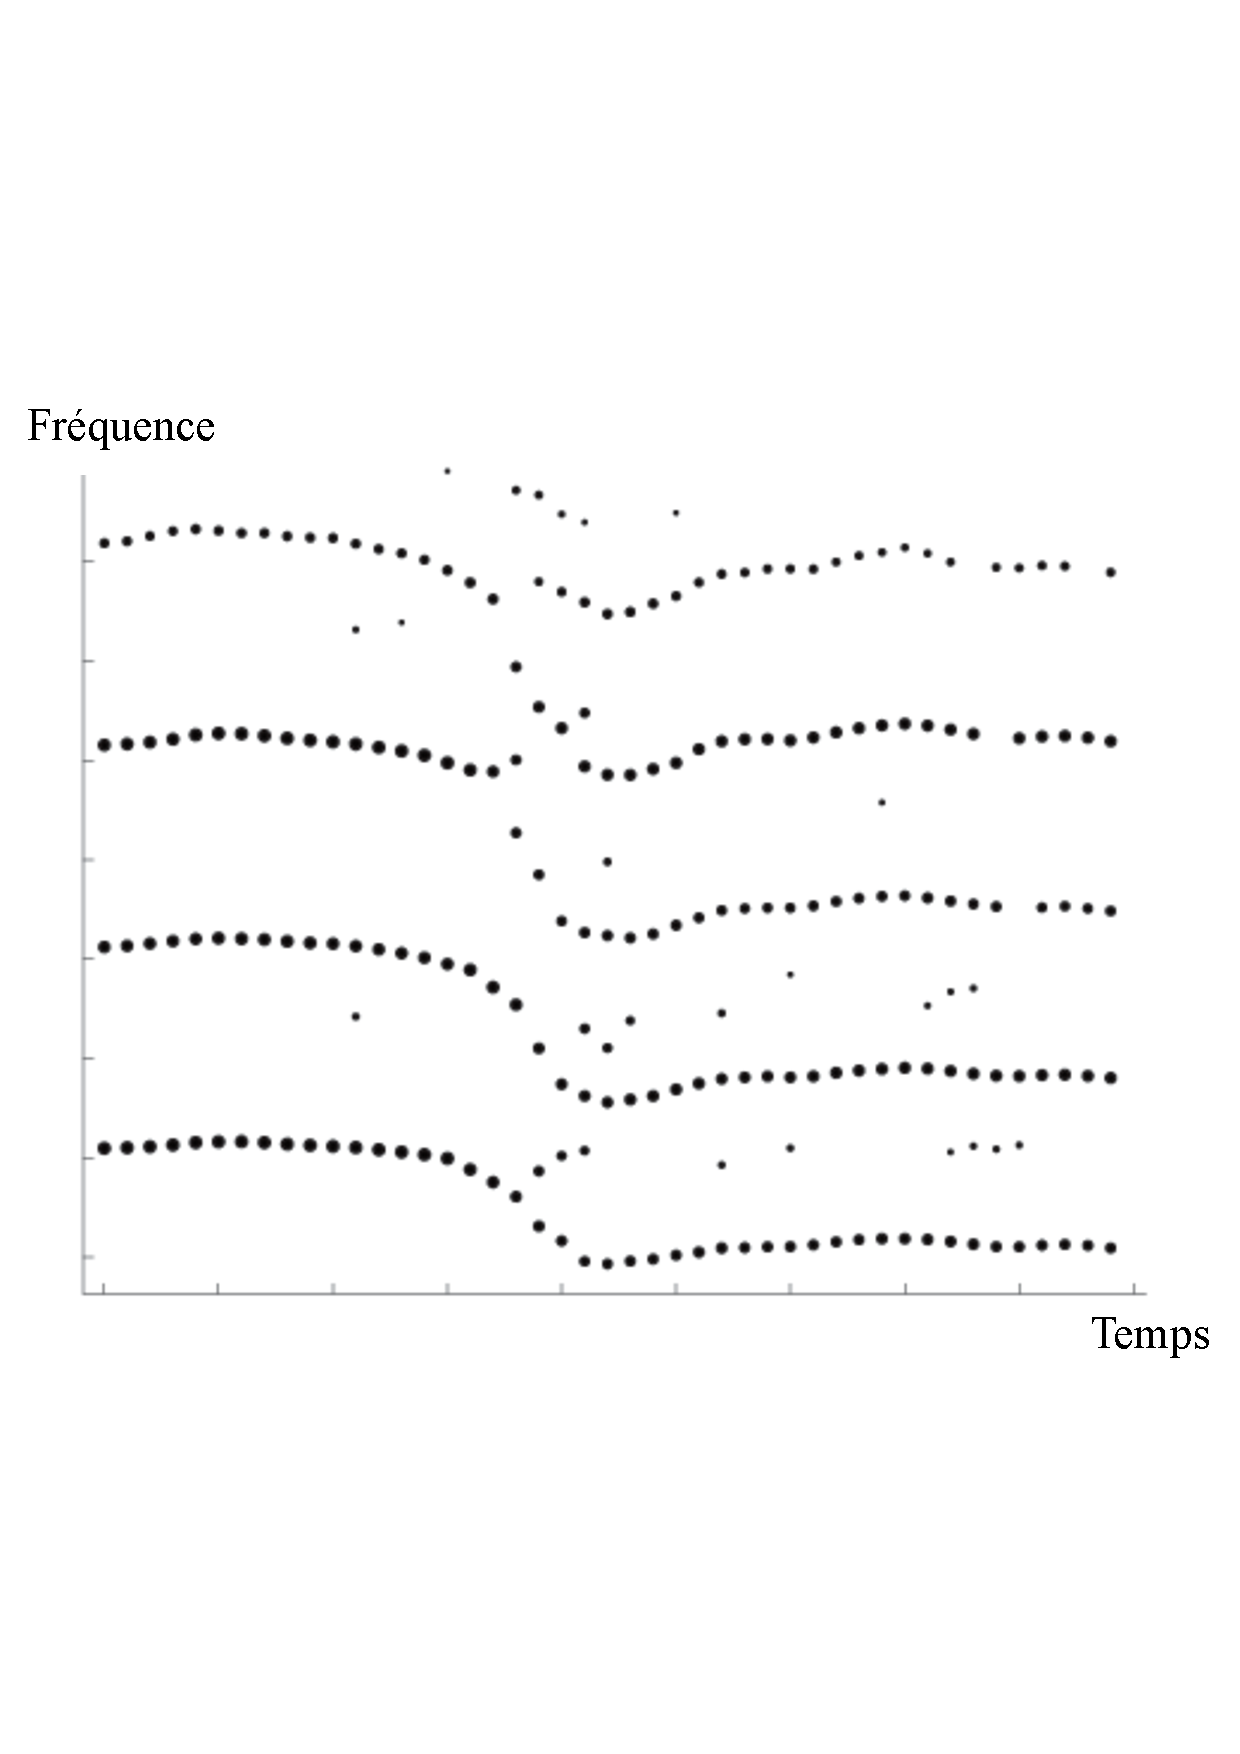
\includegraphics[width=.3333\textwidth]{voice_2048_512xp}
  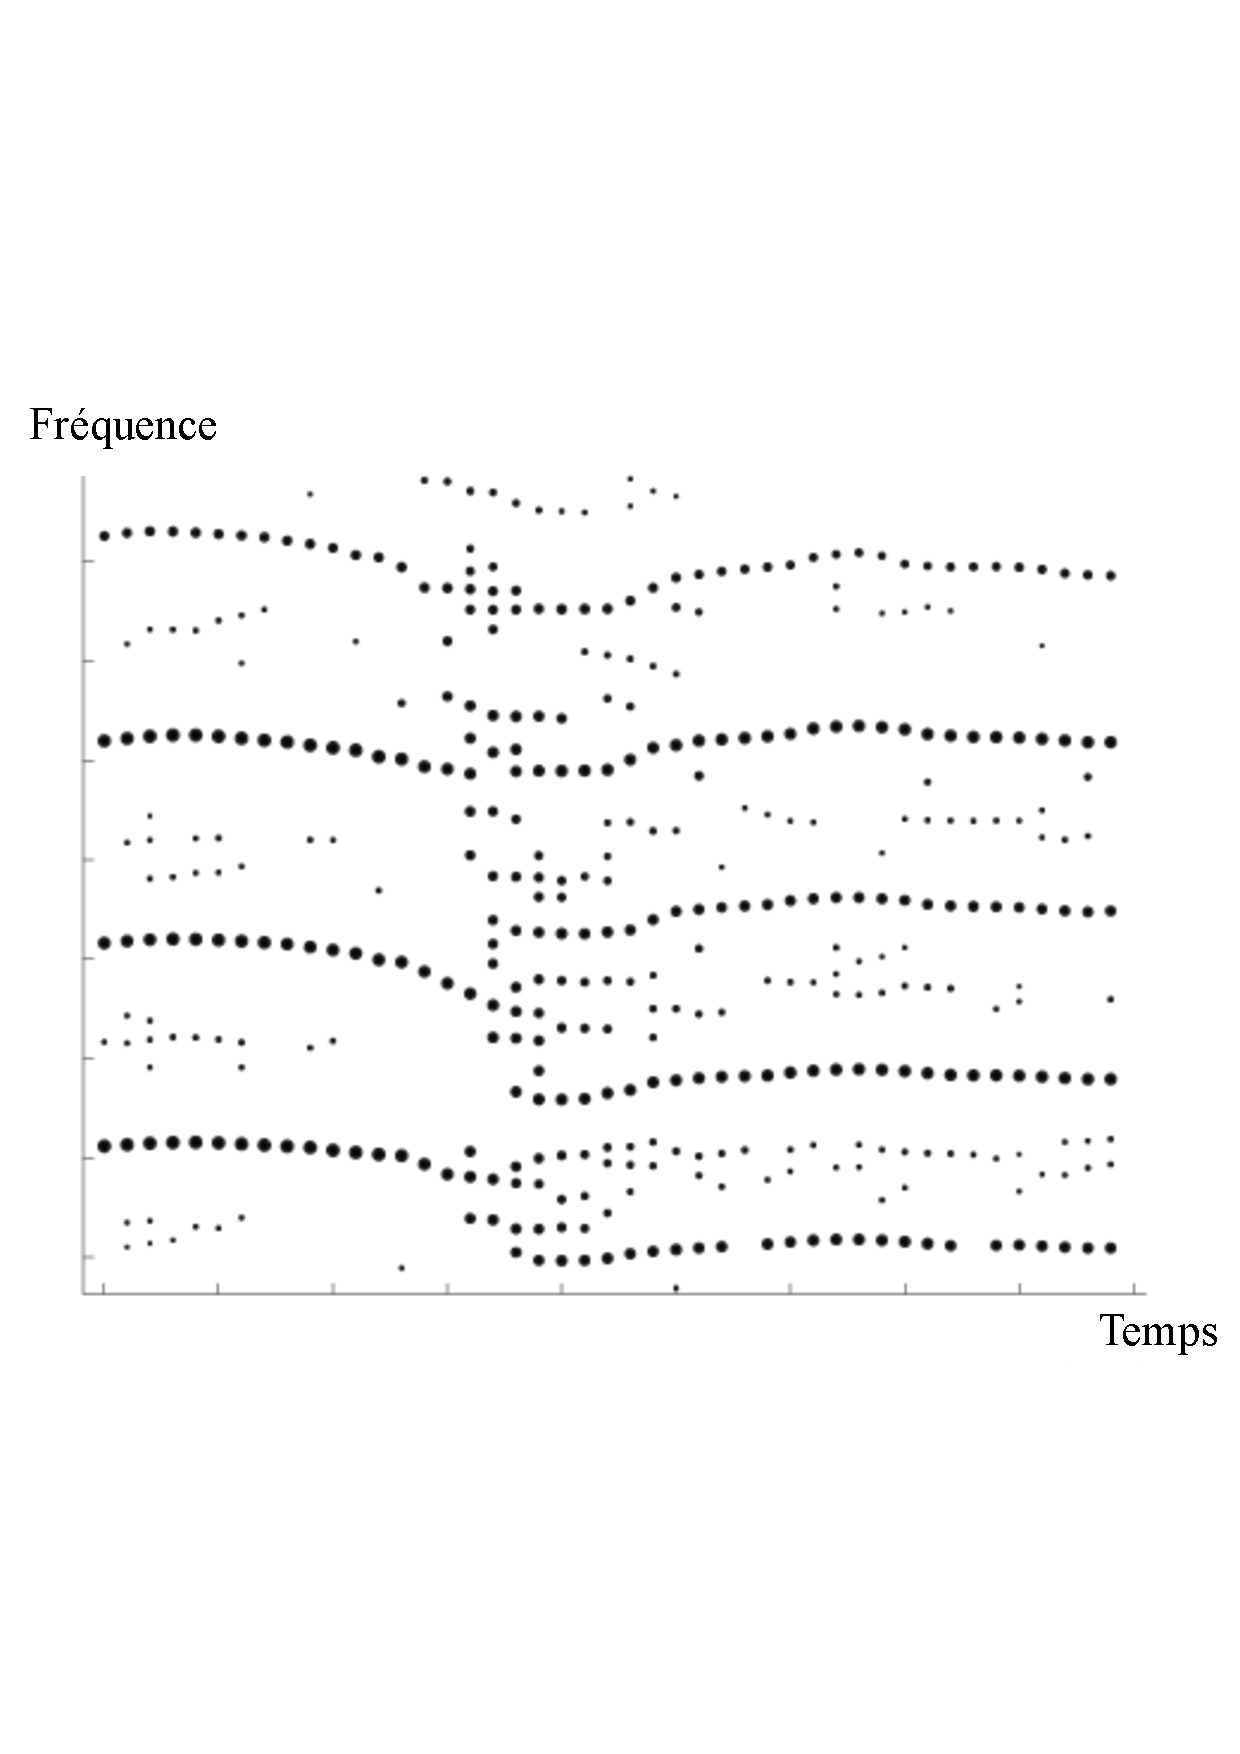
\includegraphics[width=.3333\textwidth]{voice_4096_512xp}
  \caption{Influence de la taille de fenêtre de la TFCT utilisée pour estimer un modèle sinusoïdal à court terme. De gauche à droite, la taille est de 25, 50, et 100ms, pour un pas d'avancement de 10ms.}
  \label{fig:ct}
\end{figure*}

Dans notre présentation des algorithmes d'estimation des paramètres long terme, on supposera que le signal analysé est composé d'une ou plusieurs sources dont une grande partie de leur énergie peut être correctement approximée par ce modèle. On fera également état ici des approches dites de \og restauration \fg de continuité, qui considèrent connu un modèle court terme du signal analysé mais dont la fiabilité n'est pas pré supposée\sidenote{L'application des techniques d'estimation comme celle du filtrage particulaire pour l'estimation conjointe des paramètres court terme et long terme proposée par Corentin Dubois\cite{dubois2007joint} constitue une alternative d'intérêt.}. En effet, certains artefacts dans la représentation à court terme nécessitent un traitement algorithmique approprié pour une bonne estimation des paramètres long terme. On voit par exemple sur la Figure \ref{fig:ct} l'impact de l'augmentation de la taille de fenêtre de la TFCT utilisée pour identifier les composantes à court terme.

On considère donc ici une version échantillonnée du modèle de l'équation \ref{} :
\begin{equation}
\mathcal{P}_{p}=\left(\mathcal{P}_{p}[n]\right)_{n \in\left[b_{p}, \cdots, b_{p}+l_{p}-1\right]}
\end{equation}
où chaque composante court terme se décrit comme suit :
\begin{equation}
\mathcal{P}_{p}[n]=\left(n, \phi_{p}[n], a_{p}[n], \omega_{p}[n]\right)
\end{equation}

Si nécessaire, le passage de cette version échantillonnée à la version continue pouvant se faire par interpolation.

Dans l'article séminal de George Mac Aulay \& al \cite{mcaulay}, il est donc proposé \og d'identifier \fg ces composantes long terme en reliant entre eux des atomes de trames successives. L'algorithme proposé est itératif. Supposant un ensemble de composantes long terme à la trame $t$, on va chercher à prolonger ces composantes à la trame $t+1$ en commençant par la composante de plus basse fréquence, tel que la différence entre $$ et $$ est minimale :
\begin{equation}
\left|\omega_{p}[k+1]-\omega_{p}[k]\right|<\Delta_{\omega}
\label{eq:cst}
\end{equation}
Dans un principe d'allocation exclusif, cet atome est dès lors réservé, indisponible pour la suite du déroulement de l'algorithme. Chaque atome non réservé devient alors une composante long terme qui sera potentiellement prolongée aves des atomes de la trame suivante.

On constate ici que la structure de données se complexifie sensiblement par rapport à la plupart de celles introduites avec des outils de traitement du signal canoniques, amenant une approche plus \og informatique \fg à une problématique de traitement du signal. Cette modélisation plus \og riche \fg a permis une flexibilité de manipulation qui a donner lieu à un large ensemble d'heuristiques qui ne seront pas étudiées ici, même si elles ont leur intérêt pour la qualité du rendu sonore de ce type d'approche.

La contrainte exprimée par l'équation \ref{eq:cst} favorise des trajectoires fréquentielle constantes. Dans le cas d'un modèle court terme de bonne qualité, par exemple dans le cas d'un signal monophonique à structure harmonique cette heuristique peut être raisonnable. Dans le cas de signaux bruités et/ou polyphoniques, il est utile d'améliorer la finesse du prédicteur en considérant par exemple un prédicteur linéaire appliqué aux séries temporelles des paramètres long terme. Le faible échantillonnage de ces séries temporelles nécessite des estimateurs adaptés comme celui de Burg\cite{burg1968new}.

La contrainte d'évolution lente des paramètres dans le cas d'un modèle stationnaire (prédicteur constant) se traduit naturellement par un seuil sur le delta de fréquence. Dans le cas d'un modèle non stationnaire des paramètres long terme, on trouve un gain à considérer une analyse spectrale de ces évolutions possible pour mieux déterminer les continuations à effectuer. Parmi les nombreuses continuation possibles, la continuation qui engendre le moins de hautes fréquences est privilégiée. Là encore, du fait du faible échantillonnage des paramètres, des outils d'estimation spectrale spécifiques sont nécessaires.

\begin{marginfigure}
  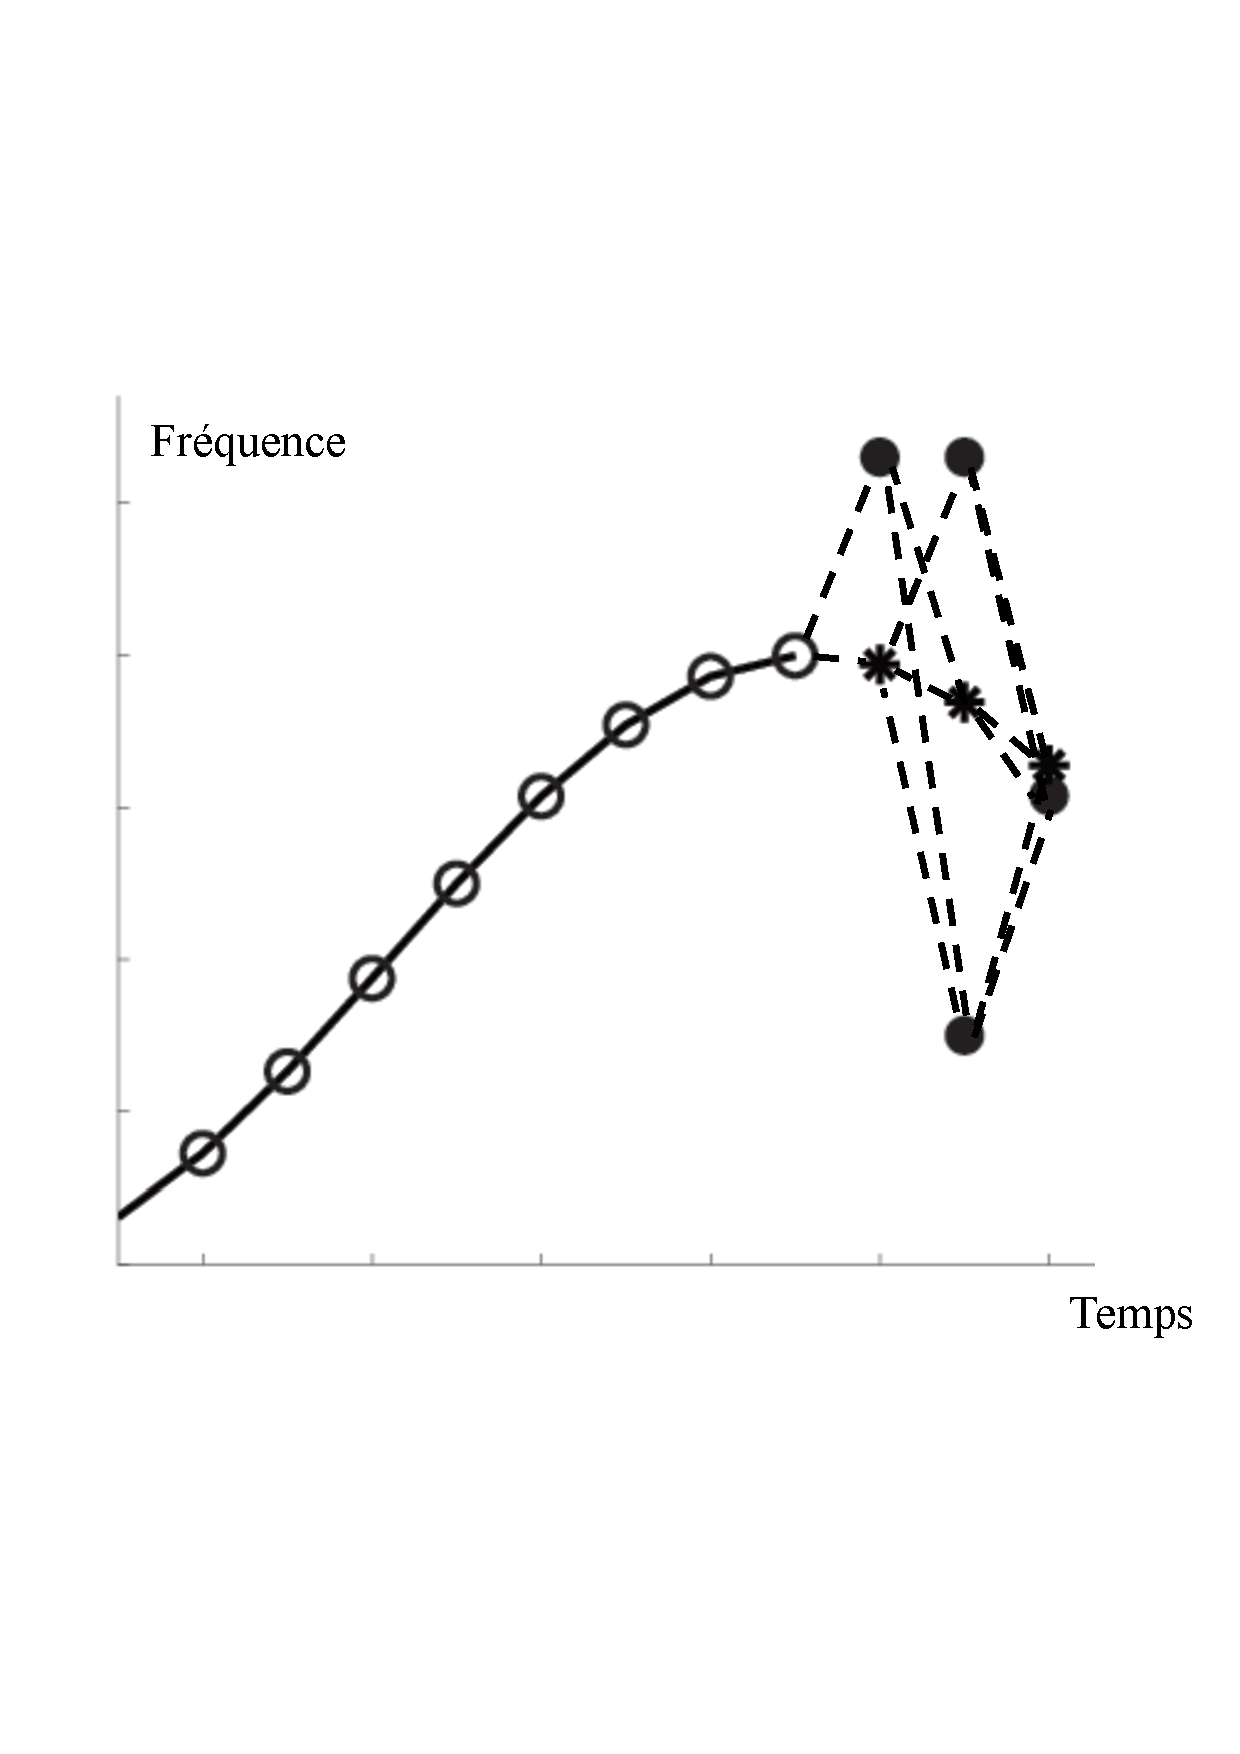
\includegraphics[width=\textwidth]{trackingxp}
  \caption{Une étape de continuation. Parmi les atomes proches (point noirs) de la prédiction (étoiles), on sélectionne la continuation qui engendre le moins de hautes fréquences dans l'évolution des paramètres de fréquence et d'amplitude.}
  \label{fig:tracking}
\end{marginfigure}

Les bons résultats en terme de rendu sonore obtenu par cette chaîne d'analyse dans le cas  de la modélisation long terme sous contrainte de débit\cite{lagrangeTaslp06} et l'interpolation de données manquantes\cite{lagrangeJaes05}, montre l'intérêt de la modélisation des modulations long terme, au moins du point de vue perceptif.

Fort de cette observation, Martin Raspaud a étudié un modèle long terme hiérarchique qui permet des manipulations riche comme par exemple de l'étirement temporel de notes vibrées\cite{raspaud2007modeles}. Le principe est de considérer les paramètres long terme comme des signaux, eux mêmes modélisables comme des sinusoïdes dont les paramètres évoluent, cette fois ci, très lentement en fonction du temps. Il est alors facile de contrôler les modulations comme le vibrato ou le tremolo.

D'une grande élégance formelle, d'une expressivité inégalée, le modèle long terme n'a pas pu trouver un large spectre d'application du fait d'un défaut clair de versatilité. Ce même handicap s'est retrouvé dans le domaine du codage où ce type de modèle\cite{den2002parametric} n'a pas réussi à concurrencer les approches TCDM. Certaines approches, dites hybrides, consistant à combiner un modèle long terme avec un modèle de bruit et modèle de transitoire ont été proposées pour tenter de palier à ce défaut. On tombe malheureusement alors dans un problème de sélection de modèles qui est à mon avis intractable, je ne détaillerai donc pas ces approches.

\marginnote{
\begin{tikzpicture}[scale=0.8, label distance=1.5mm]
  \coordinate[label=below:Fidélité]  (A) at (0,0);
  \coordinate[label=below:Versatilité] (B) at (4,0);
  \coordinate[label=above:Expressivité] (C) at (2,3.464);
  \draw [line width=1.5pt] (A) -- (B) -- (C) -- cycle;
  \draw [blue, fill=blue, line width=1.5pt] (1.4,1.8) circle [radius=.1 cm]; % slt
  \end{tikzpicture}
  Le modèle sinusoïdal à long terme est expressif et fidèle pour un champ réduit de signaux sonores.
}



\section{ \nmu Temps / fréquence / modulations}  \label{sec:tfm}

S'il est clair que la décomposition fréquentielle est de première importance, la manière dont l'énergie est modulée au court du temps au sein de ces bandes de fréquences l'est également \marginnote{On peut citer pour exemple le son éminement désagréable d'un moteur thermique deux temps (type mobylette) qui part son mouvement mécanique induit une modulation typique.}. L'importance perceptive de ce type de modulations dans notre jugement du réalisme d'un stimuli sonore est particulièrement bien exemplifiée par un stimuli synthétique produit par John Chowning. Dans ce stimuli, des sinusoïdes d'amplitude et fréquence au début constantes sont ensuite modulées par un signal synthétique composé d'une composante sinusoïdale (pour le vibrato) auquel se sur-ajoute une composante stochastique. Ce signal modulant est ensuite mis à l'échelle pour chaque harmonique. Il est important de considérer que même si ce signal modulant a été judicieusement choisi, il n'est pas issu d'un processus d'estimation à partir de signaux réels.

L'écoute montre clairement que le caractère naturel, voisé, est sensiblement plus élevé avec l'ajout de la modulation et surtout de la composante stochastique \footnote{Ce stimuli est disponible ici \url{http://webpages.mcgill.ca/staff/Group2/abregm1/web/snd/Track24.mp3} pour écoute sur le site de Al Bregman dédié à l'ASA. Les spécificités techniques du processus de synthèse sont décrites ici : \url{http://webpages.mcgill.ca/staff/Group2/abregm1/web/downloadstoc.htm\#24}.}.

\subsection{Modèles perceptifs}

Complétons nos connaissances en prenant cette fois ci, non plus un point de vue psycho-perceptif mais physiologique. L'étude des éléments physiologiques en charge du traitement de ces modulations est relativement récente car probablement sensiblement plus difficile a investiguer. On a néanmoins une bonne confiance dans le fait que le système auditif des mammifères dispose d'éléments de traitement dédiés à cette tâche. On peut notamment citer le modèle de Torsten Dau\cite{dau1997modeling} et celui de Shihab Shamma\cite{fritz2003rapid} qui étend le modèle de Dau en ajoutant une troisième dimension : l'échelle.

Shihab Shamma a étudié certains neurones du cortex auditif primaire du furet, plus particulièrement ce que l'on appelle leur champs de réponse spectro/temporellle ou "spectro-temporal receptive fields" (strf). L'animal est contraint au niveau du crâne, et par opération chirurgicale, une aiguille permettant de mesurer l'activité électrique est insérée dans le crâne de l'animal et judicieusement placée. Par exposition d'un ensemble de stimuli comportant des modulations, il est alors possible de mesurer ces strf. Au vu de ce type de réponses, Un modèle de traitement de signal est ensuite proposé.

Dans ce modèle, le signal est donc tout d'abord décomposé sur l'axe fréquentiel. La sortie est un équivalent du spectrogramme qui est ensuite décomposé une nouvelle fois fréquentiellement en temps et en fréquence grâce à des ondelettes bi-dimensionnelles paramétrées avec un facteur d'échelle. La dimension de l'échelle permet de définir le nombre de bandes qui sont conjointement utilisées pour effectuer cette seconde analyse fréquentielle.

Ces modèles sont bien entendu sujet à débat dans la communauté de neurophysiologie. Par exemple, le facteur d'échelle est pour Dau non nécessaire pour expliquer les données recueillies grâce à son protocole expérimental.

\subsection{\nmu Scattering d'ondelettes}  \label{sec:scattering}

En prenant un point de vue mathématique cette fois ci, Stéphane Mallat a proposé un modèle conceptuellement proche du modèle computationel des STRF proposé par Shihab Shamma. En mathématiques appliquées, et plus particulièrement dans le domaine des sciences des données, on cherche à construire des représentations qui aient de bonnes propriétés d'invariance et de stabilité aux déformations. C'est à dire que l'on souhaite que pour une représentation $\phi(x)$ d'un signal $x$ et d'un signal déformé $\tilde x$ :
\begin{itemize}
  \item invariance : $\phi(\tilde x) = \phi(x)$
  \item stabilité : $ \vert \phi(\tilde x) - \phi(x) | < \epsilon $
\end{itemize}

Précisons ces notions en prenant quelques exemples. Lorsque l'on cherche à reconnaitre l'instrument de musique qui a joué la note enregistrée, on souhaite généralement disposer d'une représentation du signal de cette performance qui soit invariante à certains aspects de la performance comme :
\begin{enumerate}
  \item un changement d'amplitude
  \item une translation en temps
  \item un étirement en temps
\end{enumerate}
En effet, pour la tâche pré-citée, que la note ait été jouée plus ou moins proche du microphone\sidenote{J'écarte ici pour la simplicité du discours les aspects de nuances qui ont une influence non négligeable sur le timbre.}, à un instant donné ou quelques secondes plus tard, à une hauteur donnée ou une autre, pour une durée plus ou moins longue ne devrait pas modifier de manière trop sensible notre représentation.

L'invariance au volume est obtenue de manière triviale en normalisant les signaux que l'on souhaite comparer. L'invariance locale à la translation en temps se traduit dans le domaine de Fourier en une invariance à la translation de phase par la prise du module. On souhaite généralement que l'invariance au volume et à la translation soit complète. En ce qui concerne l'invariance à l'étirement temporel, on souhaite généralement plus que la représentation soit stable à la déformation.

Il est clairement explicité dans\cite{anden2014deep} pourquoi le spectre de magnitude de Fourier n'est pas stable à même un petit étirement temporel. En effet, l'impact de l'étirement selon l'axe des fréquences n'est pas le même. Si un petit étirement déplacera d'une petite quantité les fréquences basses, les fréquences plus élevées le seront beaucoup plus. Prenons l'exemple' d'un signal harmonique de fréquence de fondamentale $440 Hz$, un étirement temporel va réduire la valeur de cette fréquence à disons $430 Hz$ pour un delta de $10 Hz$. Ce delta sera $n$ fois plus grand pour la $nième$ harmonique soit $100 Hz$ pour la dixième harmonique. Pour une transformée de Fourier avec des paniers d'une dizaine de Hertz, la différence entre les deux spectres va croitre très rapidement avec delta car l'énergie des harmoniques supérieures va très vite sortir des paniers où l'énergie des harmoniques se plaçait initialement.

Pour être plus stable à ce type de déformation, il convient alors de \og délocaliser \fg les hautes fréquences de manière plus conséquente que les basses. Suivant les communautés, on obtient cette délocalisation progressive sur l'axe des fréquences avec des transformées à Q constant, de type tiers d'octave (acoustique), des Mels ou des Barks (parole)\marginnote{Cette étude est à mon sens d'importance, car elle permet de placer un cadre mathématique pour mieux expliquer ce qui a été empiriquement vérifié dans de nombreux domaines du traitement de l'audio et motivés jusqu'ici par des arguments essentiellement neuro mimétiques.}.

En se plaçant dans le cadre des ondelettes, on obtient ce type de représentation en délocalisant en temps toutes les bandes de fréquence ce qui induit une perte d'information qu'il convient de compenser. Le principe du scattering permet de répondre élégamment à ce problème en cascadant des opérations de décomposition et en utilisant chaque niveau de décomposition pour produire une représentation compacte et informative. En dissociant ainsi décomposition et représentation, on peut préserver certaines propriétés d'intérêts comme par exemple l'inversibilité pour la décomposition et la stabilité pour la représentation.

Le scattering d'ondelettes au premier ordre est équivalent en termes conceptuels à une transformée à Q constant. En décomposant les sorties un banc de filtres en ondelettes avec un autre banc de filtres, on capte alors l'information de modulation, \textit{i.e.} comment l'énergie fluctue dans une même bande fréquence. On a vu précédemment l'importance de ce type de modulation pour la perception. Il est donc opportun de d'étudier l'apport du second ordre pour une représentation riche du signal sonore.%\marginnote{Le processus de cascade. Le troisième ordre est conceptuellement difficile à appréhender et a encore été peu étudié, pour les raisons suivantes 1) pratique : l'énergie au troisième ordre est très faible, 2) neuro-mimétique : aucun modèle perceptif n'explicite un troisième ordre de traitement.}.

L'apport du second ordre a été démontré expérimentalement pour des tâches de modélisation\cite{anden2014deep}. Nous avons complétés cette investigation en considérant une tâche pertinente pour notre propos : l'étude de la représentation des sons d'instruments de musique du répertoire en considérant des modes de jeux étendus. En effet, si la reconnaissance de l'instrument est considérée comme un problème résoluble par une représentation à Q constant, la reconnaissance du mode de jeu, et par la même d'une notion plus fine de la notion de timbre musical, comporte des éléments de modulations qui ne sont pas aisément capturés par une représentation à Q constant ou un scattering d'ondelettes à l'ordre un\cite{lostanlen2018extended}.

En terme d'architecture de décomposition, le scattering suit une organisation de type réceptive, fréquence d'abord et temps ensuite. On verra dans la partie suivante un modèle prenant une approche de type source / filtre donc temps et fréquence ensuite et qui est à ce titre plus directement tourné vers la synthèse.

\section{ \nmu Synthèse modale}

En se référant plutôt aux processus physiques de production sonore, les approches modales permettent de proposer des modèles effectifs. Ces modèles se basent sur un modèle de production de type source / filtre, où la source est généralement décrite en terme de propriétés temporelles, et le filtre en terme de propriétés fréquentielles. Pour un signal de parole, on considèrera que la source peut être soit un train d'impulsions résultant de l'ouverture périodique de l'organe phonatoire nommé, à tort,  cordes vocales pour la production des sons voisés (voyelles) soit un signal stochastique résultant de la compression du flux respiratoire pour la production des sons plosives ou sifflants (consonnes).

Le modèle source / filtre décorrelle donc naturellement la contribution de l'excitateur et celle du résonateur, ce qui est particulièrement attrayant lorsque l'on recherche un modèle de son permettant une bonne capacité d'interaction. Pour peu que les modèles utilisés pour les deux parties (source et filtre) soit bien adaptés, on obtient des modèles de sons qui sont souvent fidèles et expressifs\cite{aramaki2006analysis}. Nous avons étudié ce type de modèle pour la synthèse de sons de roulements. Ces sons présentent un challenge pour ce type de synthèse car l'interaction entre la bille et la surface sur laquelle elle roule est complexe. Néanmoins, une approche basée sur ce type de modèle\cite{LagrangeTasslp10} dont le schéma fonctionnel est présenté sur la Figure \ref{fig:modal}  a donné des résultats encourageants
\cite{Murphy11a}.

\begin{marginfigure}
  \scalebox{.6}{
  
\begin{tikzpicture}[
nonterminal/.append style={join=by ->},
tip/.style={->,shorten >=1pt},every join/.style={rounded corners},
terminal/.style={
% The shape:
rectangle,minimum size=6mm,rounded corners=1mm,
% The rest
very thick,draw=black!50,
top color=white,bottom color=black!10,
font=\ttfamily},
point/.style={circle,fill=black,minimum size=2pt},
%every node/.style=draw,
line/.style ={draw, thick, -latex',shorten
  >=2pt}]
%%%%%%%%%%%%%%%%%%%%%%%%%%%%%%%%%%%%%%%%%%%%%%%%%%%%%%%%%%%

\matrix [column sep=5mm,row sep=5mm]
{
\node [point] (p1) {} ; & \node (p2) {} ; & \node [terminal] (ma) {Analyse modale} ; &&& \node (e4) {} ; \\
&& \node [terminal] (md) {Déconvolution modale} ; & \node [terminal]  (is) {Sélection des impacts}
; && \node (e3) {} ; \\
&&& \node [terminal] (im) {Modélisation} ; && \node (e2) {} ; \\
&&& \node [terminal] (id) {Deconvolution} ; & & \node (e1) {} ;  \\
};

\begin{scope}[every path/.style=line]
\path (p1) -- node [above] {$s[n]$} (ma);
\path (p2) |- (md);
\path [dashed] (ma)  -- (md);
\path [dashed] (ma) --  node [above] {$a_k, f_k$} (e4);
\path (md) |- (id);
\path (md) -- node [above] {$e[n]$} (is);
\path (is) -- (im);
\path (is) --  node [above] {$i[n]$} (e3);
%\path (im) --  node [above] {$m(n)$} (e2);
\path (im) -- node [right] {$m[n]$} (id);
\path (id) -- (e1);
\path (id) -- node [above] {$d[n]$} (e1);
\end{scope}

\end{tikzpicture}
}
  \label{fig:modal}
\caption{}
\end{marginfigure}

La source est ici modélisée comme une distribution d'impacts dont l'amplitude est modélisée par une distribution exponentielle et l'intervalle de temps entre deux impacts par une distribution gamma. En remarquant fort justement que, lorque la bille impacte fortement le médium, l'intervalle entre cet impact et le suivant augmente, Richard Kronlan Martinet\cite{conan2014synthesis} à proposé un modèle amélioré où ces variables sont modélisées de manière conjointe.

A l'intersection entre modélisation statistique et modélisation physique, dans le sens où l'architecture du modèle de son suit un modèle de production, ce type de modèle possède deux propriétés d'importance. En premier lieu, la causalité. Au niveau du modèle de synthèse, un échantillon est strictement considéré comme une composante des échantillons précédents. En second, cette approche met l'accent sur les propriétés de filtrage des composantes modales, il ne s'agit pas ici de synthétiser un signal riche à partir d'une représentation complète du signal, mais plutôt d'exploiter un modèle source / filtre avec une implantation dédiée de ces deux modules en fonction de la tâche visée.

\marginnote{
\begin{tikzpicture}[scale=0.8, label distance=1.5mm]
  \coordinate[label=below:Fidélité]  (A) at (0,0);
  \coordinate[label=below:Versatilité] (B) at (4,0);
  \coordinate[label=above:Expressivité] (C) at (2,3.464);
  \draw [line width=1.5pt] (A) -- (B) -- (C) -- cycle;
  \draw [magenta, fill=magenta, line width=1.5pt] (1.9,2.6) circle [radius=.1 cm]; % modal
  \end{tikzpicture}
  Le modèle modal est particulièrement expressif et fidèle pour un champ assez réduit de signaux sonores.
}

Malgré toutes ces bonnes propriétés, de manière peut être encore plus marqué que pour les modèles sinusoïdaux à long terme, la versatilité reste malheureusement en deçà, car le changement de structures pour la source et le filtre ainsi que leurs modes d'interactions nécessitera le plus souvent des adaptations d'ordre computationel si ces changements sont conséquents. En particulier, les interactions non linéaires sont excessivement difficiles à modéliser en raison de manque d'outils d'estimation canoniques.

%Même si ce type d'approche est utilisée de manière assez marginale, elle garde à mon sens un intérêt historique pour mettre en perspective les approches modernes décrites dans la suite.


\section{ \nmu Discussion}

\marginnote{
\begin{tikzpicture}[scale=0.8, label distance=1.5mm]
  \coordinate[label=below:Fidélité]  (A) at (0,0);
  \coordinate[label=below:Versatilité] (B) at (4,0);
  \coordinate[label=above:Expressivité] (C) at (2,3.464);
  \draw [line width=1.5pt] (A) -- (B) -- (C) -- cycle;
  \draw [black, fill=black, line width=1.5pt] (2,.3) circle [radius=.1 cm]; % raw
  \draw [olive, fill=olive, line width=1.5pt] (1.8,.8) circle [radius=.1 cm]; % spec
  \draw [brown, fill=brown, line width=1.5pt] (2.4,.6) circle [radius=.1 cm]; % wavelets
  \draw [cyan, fill=cyan, line width=1.5pt] (1.6,1.2) circle [radius=.1 cm]; % sct
  \draw [blue, fill=blue, line width=1.5pt] (1.4,1.8) circle [radius=.1 cm]; % slt
  \draw [magenta, fill=magenta, line width=1.5pt] (1.9,2.6) circle [radius=.1 cm]; % modal
  \end{tikzpicture}

  \vspace{.3cm}

  \begin{tabular}{cl}
    \tikz\draw[black,fill=black] (0,0) circle (.1 cm); & Forme d'onde \\
    \tikz\draw[olive,fill=olive] (0,0) circle (.1 cm); & Spectrogramme \\
    \tikz\draw[brown,fill=brown] (0,0) circle (.1 cm); & Ondelettes \\
    \tikz\draw[cyan,fill=cyan] (0,0) circle (.1 cm); & Sinusoïdes à court terme \\
    \tikz\draw[blue,fill=blue] (0,0) circle (.1 cm); & Sinusoïdes à long terme \\
    \tikz\draw[magenta,fill=magenta] (0,0) circle (.1 cm); & Approches modales
  \end{tabular}
}

Si l'on prend une vue d'ensemble des différents compromis pris par les modèles de sons précédemment décrit, on voit qu'il existe des compromis équilibré entre fidélité et expressivité au détriment de la versatilité et des compromis équilibré entre fidélité et versatilité au détriment de l'expressivité. Le grand défi de la modélisation sonore est donc de proposer des approches qui puissent se placer dans un compromis entre versatilité et expressivité avec une fidélité qui reste raisonnable.

\marginnote{
\begin{tabular}{cccc}
  & fidélité & versatililité & expressivité  \\
multirésolution & \blackdot  & \blackdot & \\
causal & \blackdot  &  & \blackdot \\
non linéaire & \blackdot  & \blackdot & \\
dimensionalité réduite &  & &  \blackdot \\
contrôle lent &  & &  \blackdot
\end{tabular}
}


Au vu de certains amenés durant cette présentation, quelques éléments se révèlent incontournable pour espérer relever ce défi. Tout d'abord, le modèle doit inclure des aspects de \textbf{multi-résolution} pour être à même d'exploiter au mieux. Il me paraît également incontournable que le modèle soit \textbf{causal}. La non causalité permet une plus grande flexibilité algorithmique, la perte de la causalité amène des approximations qui sont au final souvent limite les modèles en terme de fidélité, car le processus physique qui a produit le signal sonore est lui causal. De nombreuses étapes de la propagation des ondes sonores peuvent être relativement bien approximés par des systèmes linéaires. Néamoins, il est critique pour la qualité perceptive des signaux produits que le modèle puisse modéliser des processus \textbf{non linéaires}. Enfin, pour des raisons d'expressivité, il est nécessaire que le contrôle soit aisé, donc de disposer d'une \textbf{faible dimensionalité} de l'espace de paramètres et que leur \textbf{échantillonnage temporel} soit sensiblement plus \textbf{lent} que celui du signal.


resultats récents en image

critique et differenciation image / son

superposition additivite facile

accent sur la temporalite

resumé

causal non linéarité multi resolution

POSER LES PROBLEMATIQUES

NOTER LES AMELIORATIONS






\cite{wavenet}

techniques introduites initialement pixelrnn \marginnote{La précédence d'application de nouvelle technique entre le domaine de l'image et le domaine de l'audio est quasiment toujouts observée. C'est à mon avis du à deux facteurs, l'utilité et la facilité. Nombreuses sont les applications qui necessitent du traitement de l'image, notamment à cause de la prédominance du visuel dans notre approche du réel. La facilité vient de nombreux facteurs. Un premier est qu'il est plus facile d'approcher les dimensions spatiales qui sont cohérentes entre elles. Le temps est notoirement plus complexe à modéliser. Un second est que l'oeil est notoirement plus tolérant que l'oreille. On peut donner comme exemple sur ce dernier point le morphing. Une simple somme pondérée entre deux images judicieusement cadrée permet d'obtenir des résultats appréciables. Ce type de technique est ineffective en audio où le morphing est encore un problème non résolu.}.

Les résultats obtenus en terme de qualité perceptuelle nous invite à étudier cette approche novatrice qui semble apporter des réponses à la problématique non résolue d'une méthode d'analyse synthèse multi résolution qui soit à la fois fidèle, expressive et versatile.

présentation du principe de traitement de l'information.

  réseaux neuronaux, présentation avec une optique traitement du signal (LIRE PAPIER MALLAT) \marginnote{neuromimétisme structurel pour les unités et les réseaux, question du conditionnnement chimique, et des mécanismes de prédiction et d'apprentissage. Mécanismes totalement distincts dans les modèles computationnels, pas d'équivalent en neuro sciences.}

présentation de l'architecture

vocoder

certains aspects peuvent trouver des fondements dans des modèles de sons existants

causalité stricte

source filtre

conditionnement lent

Certains aspects de l'architecture sont spécifiques.

Le plus important étant que l'écoute montre l'absence d'artefacts typiques d'une chaîne de traitement spectral mono résolution comme la tfct.

question du conditionnement



Ces points, et de nombreux autres comme l'impact des fonctions de non linéarité sur la qualité du signal généré sont des questions passionnantes, largement ouvertes en terme de compréhension scientifique.

De part la qualité du traitement et la versatilité de ces approches, leur étude constitue pour moi une opportunité pour la communauté traitement du signal. C'est d'autant plus important que la communauté d'apprentissage artificiel traverse actuellement une crise de sens. Ainsi, une vision fondée sur les principes du traitement de l'information, l'équilibre entre empirique et formalisme. Tout ces éléments qui constitue les fondements du traitement du signal sont à mon avis de grand intérêt pour répondre à des questions, qui au vu du champ d'application extrêmement vaste de ces outils, dépasse les problématiques de la seule communauté des sciences des données, pour devenir un enjeu de société.


approche source filtre <> latent code

\chapter{ \nmu La méthode scientifique en sciences des données} \label{chap:methode}

Le canon en matière de méthodologie pour l'étude d'un sujet particulier nous est offert par la méthode scientifique. Issue de pionniers comme Roger Bacon\cite{bacon1878novum}, elle permet, par son bon usage, de faire une étape importante dans la qualité de notre appréhension du monde.

Si l'on cherche à remonter plus loin dans le passé, il est remarquable de constater que l'apport des penseurs grecs et romains qui est parvenu jusqu'à nous porte essentiellement sur la nature et la définition de la vérité et finalement assez peu sur la bonne manière de l’obtenir. On trouve par contre des éléments en Orient sur cette période, comme le rapporte ce dialogue attribué à Bouddha et un de ses disciples \marginnote{Question : "Maître, comment savoir si quelque chose est vrai ou faux ? \\
Comment savoir ce qu'il faut croire ?" \\
Réponse : "Ne croyez pas en quelque chose simplement parce que
vous l'avez entendu. \\
Ne croyez pas aux traditions simplement parce que
elles se sont transmises depuis de nombreuses générations. \\
Ne croyez pas en quelque chose simplement parce que
tout le monde en parle. \\
Ne croyez pas en quelque chose simplement parce qu'on le trouve dans vos livres religieux. \\
Ne pas croire en quelque chose simplement en vous basant sur l'autorité de vos enseignants et de vos aînés. \\
Mais après une observation minutieuse et une analyse rigoureuse,
Quand vous trouvez que quelque chose est en accord avec la raison,
Et qui est propice au bien et au bénéfice de l'un et de tous,
Alors vous pouvez l'accepter et vivre en fonction. \\
Question : \og Alors, Maître, cela signifie-t-il que nous ne devrions pas nécessairement croire ce que vous venez de répondre ? \fg \\
$K\bar{a}l\bar{a}ma Sutta$, Gautama Bouddha, 500 avJc}.

Cette traduction contient pour moi deux éléments importants : 1) son exposé simple du caractère fondamentalement mal posé de la quête de la vérité, 2) le caractère résolument pragmatique de sa résolution de la \og tension sceptique \fg. Face à l'absence de référentiel non discutable permettant de confirmer ou d'infirmer une thèse, même après tout le soin que l'on peut apporter à notre argumentation, et seulement si l'on peut démontrer son intérêt pour la communauté, on peut choisir de vivre avec si tel est notre souhait, ce choix restant éminemment personnel.

C'est donc l'observation minutieuse et l'analyse rigoureuse qui va fournir le fondement de cette prise de décision. Il est donc capital de disposer de protocoles solides pour réaliser nos expériences. Et il est pour cela important de prendre conscience que la manière dont on considère une pratique impacte nécessairement cette pratique. Cet aller et retour entre (i) pratique expérimentale et (ii) observation critique de cette pratique, constitue un facteur qualitatif déterminant pour le succès de la recherche moderne.

Cela s'incarne pour moi très bien dans la relation encadré / encadrant, par exemple dans le cas d'une thèse de doctorat. Le doctorant, poussé par la force de la jeunesse, dispose d'un potentiel conséquent et d'un enthousiasme qui lui permet d'avancer malgré les nombreuses déconvenues qui sont le quotidien du chercheur. Sans vision globale de l'état des connaissances de la communauté et sans vision critique, de haut niveau, du travail effectué, il y a de fortes chances pour que les échecs restent les conclusions de ces efforts. C'est la fonction importante de l'encadrant que de mettre en perspective le travail effectué et de le placer judicieusement pour apporter de la connaissance à la communauté visée.

Néanmoins, il est à mon sens important que l'encadrant soit, sur d'autres projets l'encadré et qu'il garde un contact avec l'expérimentation, car sans cela, ses connaissances critiques resterons en arrière par rapport aux avancées de la pratique expérimentale\footnote{C'est le luxe des chercheurs confirmés que de pouvoir tenir ces deux rôles.}. \'A ce titre, je trouve personnellement plus riche et plus efficace de mettre en place des structures d'encadrement informelles lorsque je suis en charge d'une investigation.

Quels sont les savoirs nécessaires pour critiquer de manière constructive un cycle de la méthode scientifique ? C'est bien connu, acquérir des connaissances sur une pratique peut se faire en pratiquant, si possible avec des personnes reconnues dans cette pratique. Il est sans doute vain de vouloir formaliser complètements ces savoirs, néanmoins, ne serais ce que peut être pour mieux les maîtriser et les transmettre, je me suis intéressé à ce problème pendant plusieurs années.

Les solutions que j'évoque dans ce chapitre m'ont été particulièrement utile et je pense qu'elles pourront profiter aux communautés scientifiques auxquelles j'ai eu le plaisir de contribuer et plus largement dans ce que l'on appelle aujourd'hui \og les sciences des données \fg, où j'ai pu observer des phénomènes récurrents qui sont, à mon sens, néfastes pour le bon accroissement de la connaissance. Je citerai par exemple :
\begin{enumerate}
  \item l'absence de formalisme expérimental canonique et rigoureux; ce qui permet d'orienter et de justifier son effort de recherche à peu de frais;
  \item l'ajustement aux données, que ce soit par des approches algorithmiques de types série de peignes, ou de méta paramétrisation; ce qui amène le plus souvent à la production de données quantitatives coïncidentes et des conclusions qualitatives dont les bases expérimentales sont fragiles.
\end{enumerate}

Il n'est pas question d'accuser l'ensemble de la communauté de \og piper les dés \fg de manière ouverte. Ce sont des problèmes profonds qui ont leurs sources dans le fait que la recherche est effectuée par des être humains dans un contexte social donné, avec des moyens qui sont ce qu'ils sont et qui sont alloués de la manière dont ils sont alloués. Par exemple, la manière qu'un chercheur doit se comporter pour être reconnu et gérer sa carrière dans le contexte actuel me paraît particulièrement problématique au niveau du respect d'un niveau d'éthique convenable. J'aborderai cette question dans la dernière section de ce chapitre dédiée à \lnameref{sec:pairs}.

A contrario, certains chercheurs font néanmoins l'effort de se conformer à un protocole expérimental rigoureux, pour mener une étude quantitative complète d'une chaîne de traitement donnée. Je citerai ici pour exemple le travail remarquable de YLan Boureau dans le domaine du traitement de l'image\cite{boureau2010learning}. Cette étude analyse rigoureusement l'importance des différentes composants d'une chaîne de traitement d'image, en particulier les étapes de codage et d'union. La conclusion de cette étude est la suivante : \marginnote{Bien que de nombreuses recherches aient été consacrées à la conception du meilleur module de codage possible, nos résultats montrent qu’avec la classification linéaire, passer d'une étape d'union par la moyenne à une étape d'union par le maximum augmente davantage la précision que le passage de la quantification classique au codage parcimonieux. Ces résultats pourraient servir de lignes directrices pour la conception de futures architectures.}. "While much research has been devoted to devising
the best possible coding module, our results show that with
linear classification, switching from average to max pooling
increases accuracy more than switching from hard quantization to sparse coding. These results could serve as guidelines for the design of future architectures."

Pour bien comprendre l'importance de cette conclusion, il est important de placer un peu de contexte. Nous sommes en 2010, le terme de parcimonie fait couler beaucoup d'encre et de nombreuses approches utilisant ce terme comme étendard sont proposées. Cet engouement est le résultat d'une combinaison complexe de biais cognitifs, de structures sociales et idéologiques, qui amènent incidemment à concentrer l'effort de recherche d'une communauté vers ce qui semble être la bonne marche à suivre. Ce fait étant considéré comme acquis, combien d'études ne font même plus l'effort de se comparer à un algorithme de référence comme "k-means" ? Qui se pose la question de savoir si les gains obtenus à cette étape de la chaîne de traitement sont potentiellement interessant par rapport à d'autres éléments ?

Le fait est que les travaux expérimentaux de synthèse comme celui discutés ici sont rares, car ils sont coûteux en temps et finalement assez peu \og excitants \fg, pour celle ou celui qui conduit l'étude, mais surtout pour la communauté à qui ces travaux sont destinés. Avoir à remettre en question ses orientations de recherche, ses inclinaisons, ses biais, n'est pas une tâche facile, ni agréable\footnote{Cette difficulté à se remettre en question, que ce soit au niveau individuel, qu'au niveau de la communauté peut amener des difficultés considérable pour l'expression du chercheur. Je citerai ici pour exemple la réponse d'un éditeur associé d'un journal de référence dans le domaine du traitement du signal audio-numérique à la soumission d'une étude de réplication effectuée par Bob Sturm et ses collègues; réplication d'une étude publiée dans ce même journal. La réponse disait en substance que cette étude de réplication était rigoureuse et non criticable sur le fond, mais que le journal ne souhaitait pas publier des études qui mettaient en défaut des études publiées dans ce même journal.}.

On peut donc supposer qu'il est nécessaire de pouvoir comparer simplement et efficacement de nombreuses approches différentes; d'utiliser un même formalisme expérimental qui soit rigoureux et validé par la communauté. Les deux questions qui se posent alors, auxquelles je vais essayer de répondre à la lumière de ma participation à l'organisation de challenges de comparaison d'algorithmes, sont les suivantes :
\begin{itemize}
  \item est ce suffisant ?
  \item quelles sont les précautions à prendre ?
\end{itemize}

Pour répondre rapidement, je dirais que non, ce n'est pas suffisant, car la question du sens est toujours présente et doit être traitée avec des outils méthodologiques qui relèvent du questionnement scientifique. Sans prendre conscience de ce dernier point, on risque de perdre toute opportunité de faire croître la connaissance.

Les challenges tels qu'ils sont pratiqués aujourd'hui sont bien entendu une avancée incontestable par rapport à l'approche \fg mon problème, ma base de données, mon algorithme, ma métrique \og qui peut avoir son intérêt dans des phases de défrichage thématique mais qui ne peuvent être raisonnablement considérée une fois la problématique bien identifiée. Malheureusement, la mise en compétition met en exergue l'approche \og la fin justifie les moyens \fg. Au vu des objectifs le plus souvent fixé par les plupart des challenges, cela est tout à fait de bon aloi.

Pour répondre à la deuxième question, je prendrais l'exemple du mir où il est troublant de constater qu'une infime partie des publications font état de travaux effectués conjointement avec des musicologues. Or, qui connait mieux la matière que ceux qui la questionne depuis des centaines d'années ? Certes, un dialogue est nécessaire car les deux communautés sont assez disjointes, autant en terme d'objectifs, que de vocabulaire et de temporalité\marginnote{La différence de temporalité constitue dans mon expérience la plus difficile à mitiger lorsque q'un chercheur en ingéniérie cherche à collaborer avec des spécialistes de la perception ou de la cognition.}. Il est à mon avis néanmoins critique pour l'avenir de toute discipline portant sur la science des données de ne pas oublier d'où viennent ces données, que des savoirs vivants sont à notre disposition\footnote{Pour combien de temps encore ?} et que ces savoirs peuvent nous permettre de poser des questions qui ont du sens, d'apporter des réponses qui auront encore un intérêt dans une dizaine d'années et de ne pas incidemment redécouvrir des évidences \og oubliées \fg.

Au vu de ces arguments, si la question est de savoir si la conduite d'un protocole expérimental rigoureux suffit à produire de la connaissance de qualité, la réponse est négative. Elle constitue néanmoins à mon sens une condition nécessaire pour laquelle un bagage solide de connaissances sont à notre disposition pour améliorer la qualité de nos productions.

Il m'est donc apparu comme important, en parallèle de mon implication à l'interface sciences des données / perception, cognition, de revenir aux bases de la méthode scientifique pour étudier la faisabilité d'une recherche expérimentale qui soit plus rigoureuse, et ce, pour un investissement en temps qui soit réduit.

\section{ \nmu Méthodologie expérimentale en sciences des données} \label{sec:xp}

Plaçons nous dans le cadre de la méthode scientifique moderne. Elle constitue un processus itératif et cyclique dans lequel nos connaissances sont continuellement révisées à l'aide d'un algorithme constitué des composants suivants :
\begin{itemize}
  \item \textbf{Caractérisations} : observations, définitions et mesures;
  \item \textbf{Hypothèses} : explications théoriques ou hypothèses d'observations;
  \item \textbf{Prédictions} : raisonnement inductif et déductif à partir de l'hypothèse ou de la théorie;
  \item \textbf{Expériences} : évaluation de la pertinence de chacun des éléments précédents.
  \item \textbf{Revue} : mise à disposition  de la communauté des ressources nécessaires à la compréhension et la capacité de réplication des expériences.
\end{itemize}

Il est difficile de produire des recommandations qui soient pertinente pour l'intégralité des étapes de la méthode scientifique. En effet, les trois premiers composants relèvent de l'état des connaissances dans la communauté et des \og directions \fg thématiques prises. Chaque communauté scientifique doit réfléchir aux axes à privilégier, à l'allocation des ressources, etc. J'ai donc fait le choix de consacrer ma réflexion à la partie expérimentale de la méthode scientifique, les autres relevant plus d'un choix ou d'une inclinaison culturelle et politique\sidenote{Je n'exclus pas qu'il soit possible de produire des recommandations dans ces domaines, je pense simplement n'être pas assez expérimenté pour cela. La tentative serait pourtant d'intérêt.}.

Pour la partie expérimentale de la méthode, on dispose en revanche d'un ensemble fourni de méthodes et d'outils solides pour mener à bien cette étape. Ces connaissances nous proviennent essentiellement de la science du vivant (médecine et biologie) où les conclusions tirées des études effectuées ont, depuis longtemps, un potentiel important. L'impact probable qu'auront les sciences des données pour l'humanité dans les décennies qui viennent nous incitent fortement à faire de même.

Même si la tâche de systématisation est moins ambitieuse pour le composant expérimental, il est bien entendu illusoire de pouvoir proposer à la communauté un environment d'expérimentation qui soit suffisamment flexible pour permettre toutes les expériences utiles à la communauté. C'est néanmoins par ce biais que j'ai approché la question, en suivant le paradigme du \textsl{faire pour apprendre}. Durant plusieurs années j'ai donc développé un outil nommé \nameref{sec:explanes}. Cette plateforme expérimentale est basée sur une formalisation que je présenterai ici. Elle n'est probablement pas la plus élégante qui puisse être envisagée, mais elle a l'avantage d'être rompue à la pratique, où les besoins en expressivité sont dominants.



En sciences des données comme dans d'autres domaines, le principe est d'étudier la sortie $s$ d'un processus $p$ en fonction de certaines données d'entrée $d$. On souhaite que $s$ soit la meilleure possible, en fonction d'un ensemble de critères mesurables, que l'on appellera ici des \textsf
{observations} ($o$). \marginnote{\tikzstyle{stepBlock}=[draw, thick, rounded corners,
         anchor=north, align=center, rectangle split part align={center, left}, rectangle split, rectangle split parts=3]
\tikzstyle{noBlock}=[anchor=north, align=center]
\tikzstyle{stepArrow}=[->, -diamond, thick,double]
\tikzstyle{obsArrow}=[->, thick]

\begin{center}
\begin{tikzpicture}[node distance=2.1cm]

\node (1)[noBlock]{};

\node (2) [stepBlock, right=of 1]
{$p$
\nodepart{two}\tabular{@{}l}
\texttt{} \\
\endtabular
\nodepart{three}\tabular{@{}l}
\endtabular};

\node (3) [noBlock, right=of 2]{};

\draw[obsArrow]   (2.south) -- (2.south) node[midway,text width=3cm,text centered,below] {  $o$} ;
\draw[stepArrow]   (1.east) -- (2.west) node[midway,text width=1.5cm,text centered,below] {$d$} ;
\draw[stepArrow]   (2.east) -- (3.west) node[midway,text width=1.5cm,text centered,below] {$s$} ;
\end{tikzpicture}
\end{center}
 Un processus de traitement de donnees.}


A des fins de reproducibilité, on supposera que $d$ est pérenne, \textit{i.e.} n'est pas modifié par $p$. $s$ et $o$ sont non volatils, \textit{i.e.} stockés sur disque. $p$ peut éventuellement être segmenté en plusieurs étapes de traitement, qui appliquées de manière séquentielle, permettent de produire le même résultat ($s_2=s$ et $o_2=o$). \marginnote{\tikzstyle{stepBlock}=[draw, thick, rounded corners,
         anchor=north, align=center, rectangle split part align={center, left}, rectangle split, rectangle split parts=3]
\tikzstyle{noBlock}=[anchor=north, align=center]
\tikzstyle{stepArrow}=[->, -diamond, thick,double]
\tikzstyle{obsArrow}=[->, thick]

\begin{center}
\begin{tikzpicture}[node distance=1.2cm]

\node (1)[noBlock]{};

\node (2) [stepBlock, right=of 1]
{$p_1$
\nodepart{two}\tabular{@{}l}
\texttt{} \\
\endtabular
\nodepart{three}\tabular{@{}l}
\endtabular};

\node (3) [stepBlock, right=of 2]
{$p_2$
\nodepart{two}\tabular{@{}l}
\texttt{} \\
\endtabular
\nodepart{three}\tabular{@{}l}
\endtabular};

\node (4) [noBlock, right=of 3]{};

\draw[obsArrow]   (2.south) -- (2.south) node[midway,text width=3cm,text centered,below] {$o_1$} ;
\draw[obsArrow]   (3.south) -- (3.south) node[midway,text width=3cm,text centered,below] {$o_2$} ;
\draw[stepArrow]   (1.east) -- (2.west) node[midway,text width=1cm,text centered,below] {d} ;
\draw[stepArrow]   (2.east) -- (3.west) node[midway,text width=1cm,text centered,below] {$s_1$} ;
\draw[stepArrow]   (3.east) -- (4.west) node[midway,text width=1cm,text centered,below] {$s_2$} ;
\end{tikzpicture}
\end{center}
 Séparation de ce processus en deux étapes.}

Ce découpage peut se faire de manière analytique en considérant l'architecture algorithmique de $p$. En pratique, ce découpage se fait de manière à optimiser le temps nécessaire à la production de $s$ et $o$. En effet, le but de la découpe en sous tâches est de réduire le temps de calcul associé à la production de $s$ et $o$. Choisir de segmenter en deux étapes dépend d'un compromis entre le temps de calcul nécessaire à la production de $s_1$ et $o_1$ et leurs accès. En effet, si le temps nécessaire pour stocker et rapatrier $s_1$ et $o_1$ est supérieur au temps de calcul nécessaire à leur production, ce découpage n'est pas pertinent.

Le but de l'expérimentation est la confrontation de plusieurs alternatives concernant l'architecture de $p$. Nous nommerons \textsf{facteur}, un élément de conception de $p$. Chacun de ces facteurs peut prendre plusieurs valeurs, que nous nommerons \textsf{modalités}. Nous nommerons également \textsf
{condition expérimentale}, l'ensemble des modalités nécessaires à la  paramétrisation complète de $p$. Pour déterminer la condition menant à la meilleure solution, l'exploration d'un plan expérimental est pour cela nécessaire. Néanmoins, dès que l'étude dépasse la trivialité, le coût d'exécution du plan complet, \textit{i.e.} toutes les conditions expérimentales, devient prohibitif.

Une première technique consiste à effectuer l'intégralité du plan expérimental mais en simplifiant le problème à résoudre, souvent en réduisant la taille de $d$ (nombres d'exemples ou dimensions). Cette approche est risquée car elle peut amener à des choix de conception algorithmique qui ne généralisent pas correctement si le jeu de données réduit n'est pas représentatif.

Une seconde approche, plus sûre, consiste à judicieusement choisir les conditions qui nous permettent de maximiser notre connaissances de l'influence des différents facteurs, et en particulier leurs interactions. En effet, supposer que tout les facteurs sont indépendants permet de linéariser l'exploration des conditions en considérant un plan expérimental en étoile. Malheureusement, cette indépendance est rarement complètement vérifiée de manière expérimentale. Il convient alors de savoir juger ce degré d'interaction pour faire des choix éclairés. On peut pour cela utiliser des plans à facteurs réduits suivi d'une analyse de corrélations pour identifier l'importance de chaque facteur ainsi que les corrélations éventuelles entre facteurs.

Considérons un plan expérimental avec 4 facteurs $f_1$, $f_2$, $f_3$, $f_4$ ayant chacun 10 modalités ${1, 2, ..., 10}$ et un processus ayant une sortie $s=f_1*f_2+f_3+\mathbb{N}$, où $\mathbb{N}$ désigne un échantillon d'une loi normale. On considère pour simplifier ici que la sortie constitue notre observation $o=s$. Déterminer "à l'aveugle"\footnote{En considérant le processus computationel comme une boîte noire comme c'est souvent le cas.} la meilleure condition expérimentale par l'exploration du plan complet va nécessiter l'évaluation de $10^4=10000$ conditions. On cherche donc à réduire ce nombre d'évaluations nécessaire. Pour cela, on va réduire le nombre de modalités pour chaque facteur aux deux extrémums. L'exploration de ce plan expérimental va donc nécessiter l'évaluation de $2^4 = 16$ conditions expérimentales. Une analyse factorielle multivariée va permettre d'identifier l'importance des différents facteurs ainsi que leurs interactions. Comme on peut le voir sur la Figure \ref{tab:anova}, l'analyse indique une interaction entre les facteurs $f_1$ et $f_2$ et une influence nulle de $f_4$ sur notre observation. Cette connaissance nous permet de déterminer la meilleure condition avec $2^4+10^2+10=126$ évaluations, ce qui amène presque un gain d'un facteur 100 en coût de calcul par rapport au plan complet.

\begin{margintable}
\begin{tabular}{ccccc}
  & $f_1$ & $f_2$ & $f_3$ & $f_4$ \\
$f_1$  &  + & + & & \\
$f_2$  & + & + & & \\
$f_3$  & & & + & \\
$f_4$  & & & & \\
\end{tabular}
\caption{Analyse de variance du plan d'expérience réduit. Le signe $+$ indique une valeur-p inférieure à $.05$.}
\label{tab:anova}
\end{margintable}

La poursuite d'une expérimentation peut se décomposer en trois grandes étapes :
\begin{enumerate}
  \item \textbf{la conception} : conception et implantation de $p$, mise en place du plan expérimental, paramétrisation de l'environnement d'exécution, exécution de tests de conformité
  \item \textbf{l'exécution} : exécution des conditions expérimentales choisies
  \item \textbf{la réduction} : conversion des observations générées par chaque condition expérimentale
\end{enumerate}

Chacune de ces étapes a ses besoins propres en terme de ressources. L'étape de conception nécessite une capacité élevée d'interaction avec l'implantation de $p$. Il est souhaitable que $p$ puisse être exécuté localement, éventuellement avec une version réduite de $d$ pour assurer au maximum la qualité du développement de $p$ avant l'étape d'exécution et un cycle d'essai / modification qui soit le plus réduit possible.

L'étape d'exécution a pour but de réaliser la plus grande partie possible du plan expérimental demandé. L'interaction avec $p$ étant alors minimale, on peut déporter le calcul sur des machines distantes. Des possibilités d'analyse \textit{a posteriori} du déroulement de l'exécution de cette étape sont cruciales. En effet, même avec une implantation de $p$ vérifiée et validée, il est rare que cette implantation ait le comportement souhaité pour toutes les conditions expérimentales. Il est donc crucial que cela n'impacte pas le bon déroulement des autres conditions et pouvoir accéder facilement aux conditions expérimentales qui mettent en défaut l'implantation courante de $p$.

L'étape d'exécution va produire un ensemble généralement grand d'observations qu'il sera nécessaire de réduire pour produire un ensemble de données facilement manipulable, dans le but de nous informer sur le comportement de $p$ lorsqu'il est soumis à $d$. Même si le nombre d'observations est trop grand pour être appréhendé directement pour un être humain, on supposera que le volume de données est suffisamment faible pour pouvoir être manipulé localement.

%La maîtrise du temps de calcul est un point crucial de toute planification expérimentale. Cela se fait par le contrôle du temps de calcul nécessaire pour une condition expérimentale donnée, ainsi que le contrôle du nombre de conditions expérimentales.

\section{\nmu ExpLanes} \label{sec:explanes}

Le projet \explanes \marginnote{\begin{center}
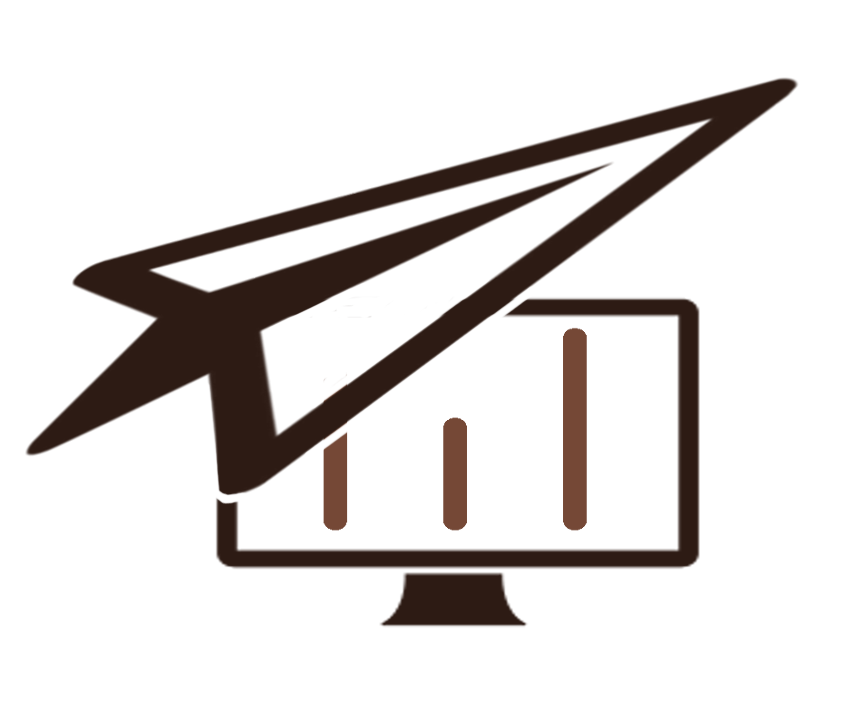
\includegraphics[width=.4\textwidth]{logoExplanes}
\end{center}
\url{http://mathieulagrange.github.io/explanes}
} est né d'une frustration grandissante de l'auteur au sujet 1) du coût de développement nécessaire à la mise en place d'un protocole expérimental de qualité, 2) l'absence de canons dans ce domaine, et 3) du risque élevé d'erreurs durant l'implantation de ce protocole expérimental compromettant sérieusement la validité des résultats obtenus. La version actuelle, écrite pour l'environnement \textsf{Matlab}\textsuperscript{\tiny\textregistered}, a nécessité trois ans de développement et est maintenant stabilisée et utilisée en production.

\subsection{Architecture}

Je présenterai cette plateforme à des fins d'illustration des concepts précédemment introduits et pour introduire des éléments nécessaire à la présentation des choix architecturaux présentés ci après.

Le principe d'\explanes est de fournir un environnement complet permettant d'aisément mettre en place un protocole expérimental destiné à répondre à des questionnements relevants des sciences des données. En particulier, il allège et systématise certaines étapes incontournables de ce type de protocole de manière à accélérer le processus de production, réduire les risques d'erreurs, et faciliter la maintenance à long terme.

Son architecture logicielle se compose de quatre composants principaux :
\begin{enumerate}
  \item un module de \textbf{commande},
  \item un module de \textbf{planification},
  \item un module d'\textbf{exécution},
  \item un module de \textbf{réduction}.
\end{enumerate}

Le module de \textbf{commande} permet de configurer l'environnement logiciel et matériel dans lequel sera exécuté la commande transmise par l'utilisateur. Toutes les commandes disponibles sont présentes à l'état statique dans un fichier de configuration qui est spécifique à chacun des utilisateurs. On peut, par l'intermédiaire de l'interpréteur modifier les valeurs de ces commandes ou en ajouter d'autres. Au sein du code de chaque étape de l'implantation du processus, cette configuration est disponible via l'objet \texttt{config}.

Le module de \textbf{planification} permet de gérer le plan d'expérience. A partir d'un fichier de description de ce plan, il génère efficacement une version manipulable. L'utilisateur peut alors aisément sélectionner les conditions expérimentales qu'il souhaite exécuter ou visualiser grâce à un mécanisme de masquage. Supposons un plan expérimental composé de 4 facteurs de 4 modalités chacune, le masque ${2 0 1}$ spécifie que la commande associée doit s'appliquer aux conditions expérimentales avec la seconde modalité du premier facteur, toutes les modalités du second et la première modalité du troisième. Le plan expérimental correspondant comprend alors 16 conditions au lieu de  $256$ pour le plan complet dont le masque implicite est ${0 0 0}$.

Le module d'\textbf{exécution} se charge, en fonction de la commande d'exécution donnée par l'utilisateur, des tâches suivantes :
\begin{itemize}
  \item séquencement des conditions expérimentales;
  \item chargement des données nécessaires et stockage des données produites;
  \item enregistrement de la progression des calculs;
  \item enregistrement des conditions expérimentales générant des erreurs.
\end{itemize}

Une fois les calculs terminés, le module d\textbf{réduction} permet, pour les conditions expérimentales sélectionnées par l'utilisateur, de :
\begin{itemize}
  \item récupérer les observations correspondantes;
  \item visualiser, par de nombreux moyens graphiques, ces observations;
  \item produire, à partir de ces visualisations, un rapport d'étude.
\end{itemize}

\subsection{\nmu Usage}

Prenons un exemple d'étude qui nous permettra d'apprécier les fonctionnalités décrites précédemment du point de vue de l'usage. Considérons que nous cherchons de manière empirique à obtenir des connaissances sur l'aire de base et le volume de formes géométriques tridimensionelles \marginnote{Le code de cet exemple est disponible\url{https://github.com/mathieulagrange/expLanes/tree/master/demo/geometricShape}}.

La création de l'expérimentation \textsl{geometricShape} se fait comme suit :
\begin{lstlisting}
expCreate('geometricShape');
\end{lstlisting}
Nous pouvons ensuite instantier deux étapes de traitement, une qui se chargera du calcul de l'aire de la base:
\begin{lstlisting}
geometricShape('addStep', 'base');
\end{lstlisting}
et une autre du volume :
\begin{lstlisting}
geometricShape('addStep', 'space');
\end{lstlisting}
Nous nous intéressons dans cette expérimentation à l'influence potentielle des différents attributs (forme, couleur, rayon, largeur, hauteur) sur l'aire de sa base et son volume. Nous considérons donc chacun de ces attributs comme des facteurs expérimentaux avec des modalités particulières.

Les formes étudiées sont le cylindre, la pyramide et le cube, nous ajoutons donc un facteur nommé \mcode{'shape'} de trois modalités :
\begin{lstlisting}
geometricShape('addFactor', ...
	{'shape', {'cylinder', 'pyramid', 'cube'}});
\end{lstlisting}
La couleur peut être bleu ou rouge, le rayon peut être de 2, 4, ou 6 mètres, la largeur de la pyramide et du cube peut être de 1, 2, et 3 mètres et la hauteur de 2, 4 ,et 6 mètres. On note ici que certains facteurs ne devront être explorés que pour une modalité d'un autre facteur. Il est en pratique très utile de pouvoir exprimer ce type d'exclusion, qui est courante dans tout plan expérimental de complexité raisonnable mettant en compétition plusieurs approches algorithmiques de paramétrisation différentes.

Le fichier statique, nommé \mcode{geshFactors.txt} pour cette expérimentation, permet de stocker les informations nécessaires à la création du plan expérimental :
\begin{lstlisting}
Factors:
1    shape =  =  = {'cylinder', 'pyramid', 'cube'}
2    color =  =  = {'blue', 'red'}
3    radius =  = 1/1 = [2, 4, 6]
4    width =  = 1/[2 3] = 1:3
5    height = 2 = 1/[1 2] = 2:2:6
\end{lstlisting}
La ligne 5 peut se lire comme suit, le facteur \mcode{'height'} n'est considéré que pour l'étape de traitement 2 et les modalités 1 et 2 du facteur 1.

Les deux étapes de traitement sont implantées comme suit. Chaque fonction responsable de chaque étape dispose de la même signature. La variable \textsl{config} expose la configuration de l'expérimentation, la variable \textsl{setting} la condition expérimentale courante, et la variable \textsl{data} expose les données produite par l'étape précédente ou les données d'entrée pour la première étape.

La première étape se charge du calcul de l'aire de la base de la forme géométrique. Pour les besoins de l'exemple, on suppose ici que $/pi$ n'est pas connu de manière précise, ce qui est simulé ici par l'ajout d'une certaine incertitude sur sa mesure :
\begin{lstlisting}
function [config, store, obs] = gesh1base(config, setting, data)

uncertainty = randn(1, 100);
switch setting.shape
    case 'cylinder'
        baseArea = (pi+uncertainty)*setting.radius^2;
    otherwise
        baseArea  = setting.width^2;
end
store.baseArea = baseArea;
obs.area = baseArea;
\end{lstlisting}

La seconde étape complète le calcul effectué par la première pour calculer le volume de la forme géométrique :
\begin{lstlisting}
function [config, store, obs] = gesh2space(config, setting, data)

switch setting.shape
    case 'cube'
       volume = data.baseArea*setting.width;
    case 'cylinder'
        volume = data.baseArea*setting.height;
    case 'pyramid'
        volume = data.baseArea*setting.height/3;
end

obs.baseArea = data.baseArea;
obs.volume = volume;
\end{lstlisting}

\begin{marginfigure}
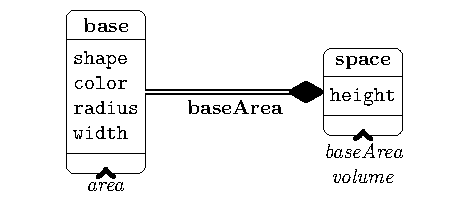
\includegraphics[width=\textwidth]{factors}
La commande \mcode{geometricShape('f')} génère un diagramme où les éléments principaux de l'expérimentation sont visibles (étapes de traitement, facteurs, données sauvegardées, observations).
\end{marginfigure}

Une fois l'implantation effectuée, le traitement est effectué avec la commande \mcode{'do'}. Par exemple, la commande
\begin{lstlisting}
geometricShape('do', 1);
\end{lstlisting}
demande le calcul de l'étape 1 pour toutes les conditions expérimentales, ici au nombre de 18. Il est souvent nécessaire de ne pas effectuer le plan expérimental complet (étude spécifique, reprise sur erreur, ...), le mécanisme de masquage est alors utilisé. Par exemple, la commande
\begin{lstlisting}
geometricShape('do', 0, 'mask', {[1 2] 0 1})}
\end{lstlisting}
demande le calcul successif des deux étapes pour les cylindres de rayon 2 et toutes les pyramides.

A la suite de la réalisation du plan complet, le répertoire dédié au stockage des données de calcul et d'observations contient : \\
\begin{Verbatim}[fontsize=\scriptsize]
	base/color: blue, radius: 2, shape: cylinder_data.mat            space/color: blue, height: 2, shape: pyramid, width: 2_obs.mat
	base/color: blue, radius: 2, shape: cylinder_obs.mat             space/color: blue, height: 2, shape: pyramid, width: 3_obs.mat
	base/color: blue, radius: 4, shape: cylinder_data.mat            space/color: blue, height: 4, radius: 2, shape: cylinder_obs.mat
	base/color: blue, radius: 4, shape: cylinder_obs.mat             space/color: blue, height: 4, radius: 4, shape: cylinder_obs.mat
	base/color: blue, radius: 6, shape: cylinder_data.mat            space/color: blue, height: 4, radius: 6, shape: cylinder_obs.mat
	base/color: blue, radius: 6, shape: cylinder_obs.mat             space/color: blue, height: 4, shape: pyramid, width: 1_obs.mat
	base/color: blue, shape: cube, width: 1_data.mat                 space/color: blue, height: 4, shape: pyramid, width: 2_obs.mat
	base/color: blue, shape: cube, width: 1_obs.mat                  space/color: blue, height: 4, shape: pyramid, width: 3_obs.mat
	...							      ...
\end{Verbatim}

Ce n'est pas explicite dans cet exemple, mais les fichiers \mcode{\_data} dédiés au stockage des données de calculs sont souvent de taille plus conséquente que les observations qui elles ont vocation à rester de taille raisonnable pour pouvoir être transférées des machines de calcul aux machines de développement et de visualisation pour pouvoir être aisément analysées. Pour toute expérimentation de taille raisonnable, les noms de fichiers peuvent également être compactés pour ne pas dépasser les 250 caractères requis par la plupart des systèmes de gestions de fichiers.

\`A la fin du traitement, les observations de la dernière étape de traitement sont affichées :
\begin{Verbatim}[fontsize=\scriptsize]
	Loaded data files dates are in the range: | 01-Apr-2019 10:15:55 || 01-Apr-2019 10:15:56 |
	    'shape'       'color'    'radius'    'width'    'height'    'baseArea'          'time'    'volume'
	    '---'         '---'      '---'       '---'      '---'       '---'               '---'     '---'
	    'cylinder'    'blue'     '2'         ''         '2'         '  12.55 (4.32)'    '0.22'    '   25.11 (8.63)'
	    'cylinder'    'blue'     '2'         ''         '4'         '  12.55 (4.32)'    '0.09'    '  50.22 (17.27)'
	    'cylinder'    'blue'     '2'         ''         '6'         '  12.55 (4.32)'    '0.00'    '  75.32 (25.90)'
	    'cylinder'    'blue'     '4'         ''         '2'         ' 50.85 (16.54)'    '0.00'    ' 101.70 (33.08)'
	    'cylinder'    'blue'     '4'         ''         '4'         ' 50.85 (16.54)'    '0.00'    ' 203.41 (66.15)'
	    'cylinder'    'blue'     '4'         ''         '6'         ' 50.85 (16.54)'    '0.00'    ' 305.11 (99.23)'
	    'cylinder'    'blue'     '6'         ''         '2'         '109.79 (33.75)'    '0.00'    ' 219.57 (67.50)'
	    'cylinder'    'blue'     '6'         ''         '4'         '109.79 (33.75)'    '0.01'    '439.14 (135.00)'
	    'cylinder'    'blue'     '6'         ''         '6'         '109.79 (33.75)'    '0.00'    '658.72 (202.50)'
	    'cylinder'    'red'      '2'         ''         '2'         '  11.92 (4.33)'    '0.00'    '   23.84 (8.66)'
	    'cylinder'    'red'      '2'         ''         '4'         '  11.92 (4.33)'    '0.00'    '  47.68 (17.32)'
\end{Verbatim}

L'accès à une grande diversité de mises en forme de l'exposition des observations utiles au discours est un élément nécessaire pour une expérimentation efficace. La plateforme \explanes dispose d'un grand nombre de fonctionnalités conçues pour permettre une certaine flexibilité dans leurs usages.

Par exemple, ce dernier affichage peut être ré-obtenu grâce à la commande suivante :
\begin{lstlisting}
geometricShape('display', 2, 'expose', '>', 'mask', {[1 2] 0 1});
\end{lstlisting}
La commande :
\begin{lstlisting}
geometricShape('display', 2, 'mask', {1 0 1},...
 'expose', {'t', 'obs', 2});
\end{lstlisting}
affiche les volumes (observations 2) de l'étape 2 pour chaque cylindre de rayon 2 triés par la première observation sélectionnée. La fonte rouge indique la plus haute valeur, et les valeurs en gras, celles qui ne sont pas statistiquement différentes, au sens d'un t-test par paires effectué entre les observations de la condition expérimentale et celle correspondant à la plus haute valeur.

\begin{margintable}
\caption{Visualisation sous forme de table \LaTeX.}
\begin{tabular}{llc}
color & height & volume \\
\hline
blue & 2 &  26.12$\pm$9.30 \\
blue & 4 & 52.23$\pm$18.60 \\
blue & 6 & \textbf{\textcolor{red}{78.35$\pm$27.90}} \\
red & 2 &  24.61$\pm$7.54 \\
red & 4 & 49.23$\pm$15.07 \\
red & 6 & \textbf{73.84$\pm$22.61} \\
\end{tabular}
\end{margintable}

Dans notre exemple, même si le cylindre bleu est plus volumineux que le rouge, cette différence n'étant pas significative, on peut en conclure expérimentalement que la couleur n'influe pas sur le volume. Une fois la phase d'analyse des résultats effectuée, nous pouvons alors communiquer les résultats grâce à la production de rapports d'expérimentation. Quelques exemples de rapports d'expérimentation pour des expérimentations plus ambitieuses sont disponibles sur le site du projet \textsl{expLanes}.

Je me suis attaché à décrire ici une contribution personnelle à une problématique d'importance qui, sans prétendre viser à l'universalité, propose une systématisation de l'étape d'expérimentation de la méthode scientifique, adaptée aux problématiques relevant des sciences des données.

Je présente dans la section suivante des éléments de réflexion concernant la revue par les pairs et comment ce type de contribution peut amener des éléments d'intérêt pour la modernisation et à la préservation des fondements de cette délicate dernière étape de la méthode scientifique.

\section{\nmu La revue par les pairs} \label{sec:pairs}

Outil indispensable à la communauté scientifique, elle comporte néanmoins des risques pour le chercheur, c'est en effet à ce moment que les fruits de son travail sont exposés, à la critique, à l'utilisation abusive, ... C'est aussi une formidable opportunité de voir son travail servir de base pour la recherche future.

On assiste actuellement à une \og crise \fg une crise de la publication d'articles, principalement à cause d'une normalisation d'une expression anglo saxonne "publish or perish" qui est, dans un nombre toujours plus grand de pays, devenue loi. Les nouveaux moyens numériques de diffusion facilitant cette inflation, le chercheur doit passer beaucoup de temps à écrire, mais aussi à relire, des articles dont le contenu s'allège en conséquence. En considérant que le nombre de personnes dédiant leur carrière à la recherche scientifique est resté stable durant ces 50 dernières années, les dernières estimations de l'évolution du nombre d'articles publiés sont préoccupantes\cite{bornmann2015growth} et posent de nombreuses inquiétudes quand à la solidité du principe de publication d'articles comme fondement de la revue par les pairs.

\begin{marginfigure}
  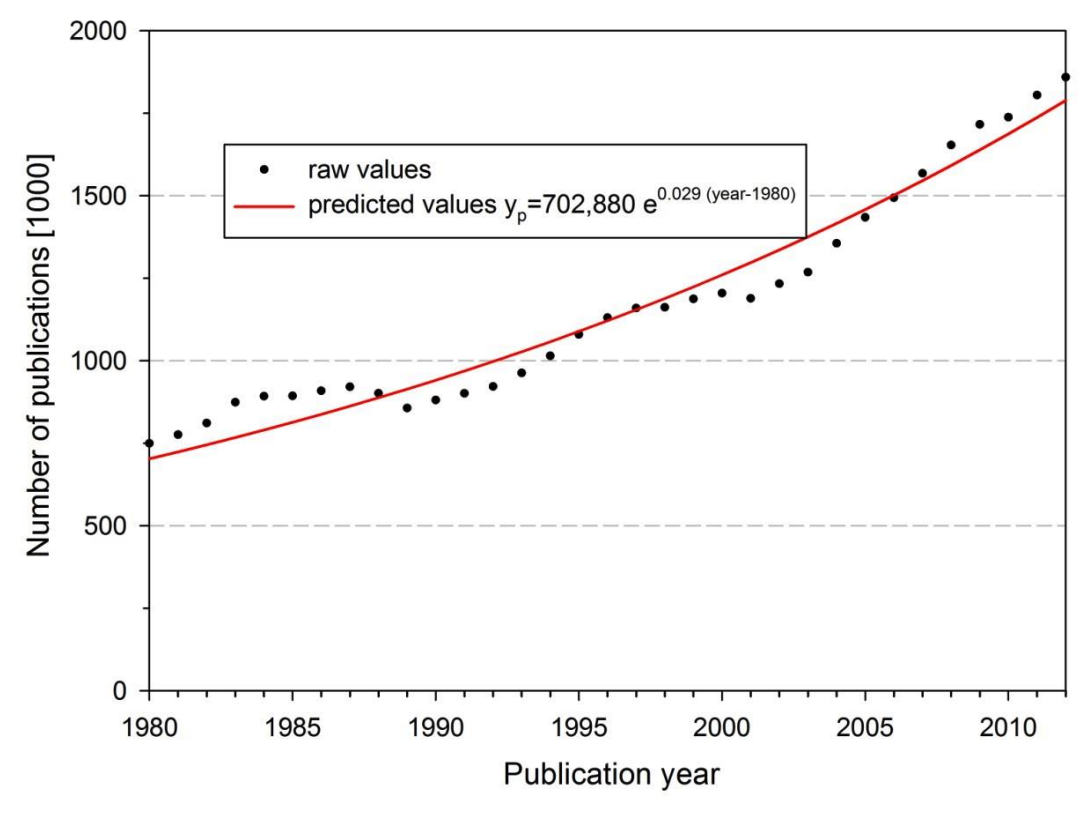
\includegraphics[width=\textwidth]{nbArticles}
  \caption{Estimation de la croissance du nombre de publications scientifiques.}
\end{marginfigure}

\marginnote{A ceci s'ajoute la position maintenant indéfendable des éditeurs qui, par abus de position historique, ne facilitent pas l'évolution nécessaire. Comment expliquer au contribuable les sommes demandées au chercheur pour l'archivage de ses articles (actuellement environ 1500 euros pour un fichier d'une dizaine de Mo). Il est malheureusement difficile pour un chercheur de prendre la décision de manière unilatérale de prendre des dispositions alternatives.}

Comme tout moment de crise, de nouvelles opportunités émergent également qui pourraient amener à une nouvelle implémentation de cette dernière étape de la méthode scientifique qui soit plus respectueuse du chercheur et également plus effective pour la communauté. \marginnote{J'éviterai ici toutes questions concernant l'évaluation du chercheur, les produits de l'étape de la revue par les pairs n'étant pas à mon sens un outil approprié pour cet objectif.}

Dans une tradition issue de la physique expérimentale, la revue par les pairs se base sur la production d'une description aussi précise que possible du protocole expérimental et d'une discussion plus ou moins approfondie sur l'interprétation que font les auteurs sur les résultats obtenus. Ce format \og article \fg est motivé par le fait que l'environnement expérimental est très coûteux à mettre en place et difficilement transposable. Par accumulation d'expériences avec des protocoles expérimentaux d'une spécificité plus ou moins contrôlée, la communauté s'approche de ce que l'on peut être raisonnable de penser être la vérité. Un exemple particulièrement illustratif de ce processus est montré sur la Figure \ref{fig:copper} montrant une série de mesures de la conductivité du cuivre en fonction de sa température. Par l'accumulation et la réduction de mesures effectuées de manière indépendante, notre connaissance du phénomène observé s'affine.

\begin{marginfigure}
  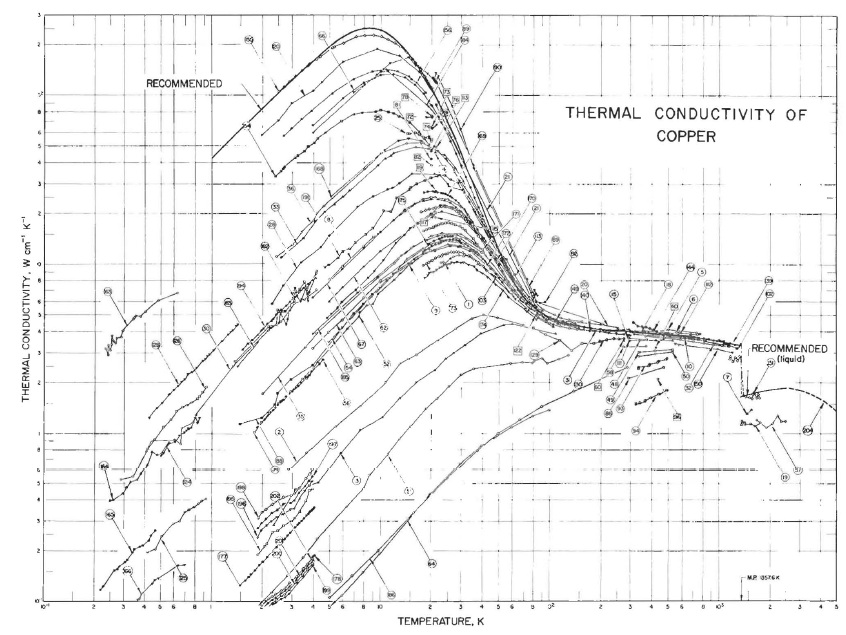
\includegraphics[width=\textwidth]{copper}
  \caption{Mesures de la conductivité du cuivre en fonction de sa température. Chaque ligne pointée par une bulle numérotée désigne les mesures publiées dans un article donné.}
  \label{fig:copper}
\end{marginfigure}

Dans le domaine de la sciences des données, on peut considérablement accélérer le processus de reproduction et d'extension, car il est plus aisé de mettre en place le paradigme de la recherche reproductible. En suivant la définition séminale de Donoho\marginnote{"An article about computational science in a scientific publication is not the scholarship itself, it is merely an advertising of the scholarship. The actual scholarship is the complete software development environment and the complete set of instructions which generated the figures." \\—D. Donoho} et en l'étendant au cadre des sciences des données, on peut considérer qu'une contribution scientifique doit pour cela être composée:
\begin{enumerate}
  \item des données servant de base à l'expérimentation;
  \item de l'implémentation qui, en fonction de ces données, produit les éléments quantitatifs discutés dans le compte rendu;
  \item d'un compte rendu d'expérience ou article détaillant les hypothèses, le protocole expérimental et les conclusions.
\end{enumerate}

Concernant la pérennité des données et de l'article, ces données numériques dites \og statiques \fg ne posent pas de challenge particulier. Ce n'est malheureusement pas le cas du code informatique car il dépend d'une pérennité de l'interprétation de ce code sur les machines contemporaines. L'archivage et la maintenance du matériel qui a servi aux expérimentations n'est pas dans le cas général envisageable. Les difficultés de réplication pour cause d'obsolescence matérielle et logicielle sont endémiques de la recherche en sciences des données car cette activité se situe généralement dans des secteurs de pointe évoluant très rapidement\marginnote{Je citerai pour exemple l'évolution actuelle des bibliothèques de calcul sur unité de calcul graphique comme la bibliothèque \textsf{cuda}\textsuperscript{\tiny\textregistered} développée par \textsf{nvidia}\textsuperscript{\tiny\textregistered}. Indispensable pour tout traitement efficace d'architectures profondes, cette bibliothèque est propriétaire et les versions antérieures ne sont plus maintenues après seulement quelques années.}.

Il reste que, bien souvent, une maintenance régulière du code par les auteurs au cours du temps permet de préserver un certain niveau d'équivalence des résultats. Il est alors pour cela très utile de disposer d'un code qui soit bien structuré et facile à maintenir. Cette maintenance sera également grandement facilitée par le choix judicieux des dépendances du code informatique publié. Si la phase d'expérimentation nous incite généralement à essayer de nombreuses approches, dont certaines très novatrices mais potentiellement instables et faiblement maintenues, il convient au moment de la publication de réfléchir à un bon équilibre entre apport technique et pérennité.

Ceci étant dit, garantir une reproducibilité complète pour un temps long de toutes ses productions est un défi probablement trop coûteux pour le chercheur. Il convient néanmoins de réfléchir en amont à cette problématique et d'allouer l'énergie nécessaire aux projets qui trouvent intérêt dans la communauté\marginnote{Les plateformes de développement collaboratif comme gitHub sont à ce titre particulièrement adaptées car elles permettent d'être informé de l'intérêt que porte la communauté aux travaux publiés et d'assister les collègues lors des tentatives de réplication.}.

Même si l'implémentation particulière n'a pas vocation à être pérenne, il est bien évident que si les auteurs ont suivi un protocole expérimental canonique avec un effort de clarté et de concision dans l'implémentation, la réplication sera bien plus accessible. L'utilisation de cadres computationnels comme \explanes pour mettre en place ce protocole expérimental est d'intérêt car ils permettent d'encourager de bonnes pratiques en facilitant leurs mises en place.

Concernant les données nécessaires à la production des résultats, il est techniquement parlant aisé que les données expérimentales soient stockées de manière pérenne sur des plateformes publiques\footnote{Les plateformes de type \textsf
{archive} (\url{https://archive.org}) ou \textsf
{zenodo} (\url{https://zenodo.org}) sont de bons candidats.}. La contrainte ici n'est pas d'ordre technique mais légale. L'usage de données publiques doit donc être encouragé par la communauté, quitte à s'éloigner du champ applicatif immédiat, où les enjeux économiques, légaux, de respect de la vie privée entrent en conflit avec les principes mêmes du questionnement scientifique.

\chapter{Parcours académique}

\begin{tabular}{ll}
{\bf  Statut actuel}: & Chargé de recherche CNRS classe normale  \\
 & - recruté en 2009 par la commission interdisciplinaire (CID) 44 \\ & \og Cognition, langage, traitement de l’information, systèmes
naturels et artificiels \fg \\ & - rattaché en 2012 à la section 07  \og Sciences de l'information \fg \\
\\
  {\bf CNU}: &
   - section 27 \og Informatique \fg \\ & - section 61 \og Génie informatique, automatique et traitement du signal \fg\\
\end{tabular}

\section{Diplômes}
\begin{tabular}{ll}
  2001 & Master Informatique : \og Accélération de la synthèse sonore \fg \\ & encadré par Sylvain Marchand, \\ & soutenu à l'Université de Bordeaux 1 \\
  2004 & Doctorat Informatique : \og Modélisation long terme des signaux polyphoniques \fg \\ & dirigé par Myriam Desainte-Catherine, Sylvain Marchand et Jean-Bernard Rault, \\ & soutenu à l'Université de Bordeaux 1 \\ & \url{https://www.theses.fr/2004BOR12917} \\ & \url{https://tel.archives-ouvertes.fr/tel-00009550} \\
\end{tabular}

\section{Carrière}
\begin{tabular}{ll}
  2001-2004 & {\bf Doctorant Université Bordeaux 1} et Ingénieur de Recherche \\
  &  à France Télécom R\&D Rennes \\
  & TECH/IRIS (équipe codage et multimédia) \\
  2004-2005 & {\bf Enseignant chercheur (ATER)} au LaBRI (Université Bordeaux 1) \\
  2005-2006 & {\bf Enseignant chercheur (ATER)}  à l'Enseirb (Université Bordeaux 1) \\
  2006-2007 & {\bf Post-doctorant} au sein du département d'informatique \\
  &  Université de Victoria, BC, Canada \\
 2007-2008 &  {\bf Post-doctorant} au sein du département de  "Music Technology"  \\
  &  Université de McGill, QC, Canada \\
 2008- 2009 &  {\bf Post-doctorant} au sein de  l'équipe  Acoustique Audio et Ondes (Aao)  \\
  & Télécom ParisTech \\
 2009-2013 &  {\bf Chercheur CNRS} au sein de l'équipe Analyse / Synthèse  \\
  & Ircam (Umr 9912), Paris \\
 2013- -- &  {\bf Chercheur CNRS} au sein de l'équipe \\
 & Signal, Images et Son (Sims)  \\
  & Ls2n (Umr 6004), Ecole Centrale de Nantes \\

\end{tabular}

\section{Participation à des projets financés}
\begin{itemize}
\item 2003 - 2004 : "Adaptive rate-distortion optimized sound coder", projet Européen (Eu grant no. IST-2001-34095)
\item 2006 - 2007 : "From the laboratory to the concert: applications of gesture research to live performance", projet Sshrc, Canada
\item 2006 - 2007 : "Graph algorithms for audio analysis", projet Nserc, Canada
\item 2007 - 2008 : "Sound and haptic synthesis", projet Européen Enactive et financement Nserc, Canada
\item 2008 - 2009 : "Décomposition en éléments sonores et application à la musique", projet Anr
\item 2009 - 2012 : "Quaero", Projet Oseo
\item 2012 - 2014 : "Computational auditory scene analysis", projet fondation sciences et technologie, Portugal
\item 2012 - 2015 : "Hierarchical object based learning", projet Anr jeune chercheur / jeune chercheuse (investigateur principal)
\item 2015 - 2017 : Projet "Traité instrumental collaboratif en ligne" (Ticel), Projet Paris sciences et lettres (Psl) en collaboration avec le Conservatoire National de Musique et de Danse de Paris (Cnsmdp)
\item 2017 - -- : "Caractérisation des environnements sonores urbains : vers une approche globale associant données libres, mesures et modélisations" (Cense), projet Anr
\end{itemize}

\section{Encadrement de doctorats}
\begin{itemize}
  \item Rémi Foucard (2010 - 2013): "Fusion multi-niveaux par boosting pour le tagging automatique", taux d'encadrement 40 \%
  \item Grégoire Lafay (2013 - 2016): "Simulation de scènes sonores environnementales : application à l'analyse sensorielle et à l'analyse automatique", taux d'encadrement 40 \%
  \item Jean-Rémy Gloaguen (2015 - 2018): "Estimation du niveau sonore de sources d'intérêt au sein de mélanges sonores urbains : application au trafic routier", taux d'encadrement 30 \%
  \item Félix Gontier (2017 - --): "Modélisation de signaux sonores par approches neuronales profondes", taux d'encadrement 30 \%
\end{itemize}

\section{Indices bibliométriques}
\begin{itemize}
\item 21 revues internationales à comité de lecture
\item 62 conférences internationales à comité de lecture
\item citations: 1615 (source Google Scholar, Mai 2019)
\item indice h: 19 (source Google Scholar, Mai 2019)
\end{itemize}

%
 \bibliographystyle{plainnat}
 \nobibliography{biblio/strings,biblio/journals,biblio/conferences,bib}
\chapter{ \nmu Notice bibliographique} \label{chap:biblio}

\begin{center}
Les publications référencées ici sont disponible au format pdf à cette adresse : \\ \url{https://mathieulagrange.github.io}
\end{center}

\nocitejournals{*}
%\nocitejournals{lagrangeTaslp08, Lagrange12a, LagrangeTasslp10, lagrangeTaslp06,  lagrangeJaes05, lagrangePrl09, lagrangeMta09, lagrangeJaes07,Murphy11a,Lagrange12c}

\bibliographystylejournals{plainyr-revnonnum}
\bibliographyjournals{biblio/strings,biblio/journals}

\setcounter{enumiv}{0}

\nociteconferences{*}

\bibliographystyleconferences{plainyr-revnonnum}
\bibliographyconferences{biblio/strings,biblio/conferences}

\setcounter{enumiv}{0}

\nocitechapters{*}

\bibliographystylechapters{plainyr-revnonnum}
\bibliographychapters{biblio/strings,biblio/chapters}

% \setcounter{enumiv}{0}
%
% \nociteworkshops{*}
%
% \bibliographystyleworkshops{plainyr-revnonnum}
% \bibliographyworkshops{biblio/strings,biblio/workshops}

\setcounter{enumiv}{0}

\nocitesoftware{*}

\bibliographystylesoftware{plainyr-revnonnum}
\bibliographysoftware{biblio/software}

\setcounter{enumiv}{0}

\nocitepatents{*}

\bibliographystylepatents{plainyr-revnonnum}
\bibliographypatents{biblio/patents}


\end{document}
